\documentclass{beamer}


\usepackage[utf8]{inputenc}   % Підтримка UTF-8
\usepackage[ukrainian]{babel} % Підтримка української мови
\usepackage[ukrainian=nohyphenation]{hyphsubst}
\usepackage[T2A]{fontenc}      % Кодова таблиця для кирилиці

\usepackage{booktabs}
\usepackage{amsmath, amsfonts} % Для математики, якщо потрібно
\usepackage{hyperref}          % Для створення посилань
\usepackage{listings}          % Пакет для вставки коду
\usepackage{graphicx}
\usepackage{csvsimple}
\usepackage{parskip}
\usepackage{csquotes}
\usepackage{xcolor}
\usepackage{multicol} % Для багатостовпчикового тексту
\usepackage{caption}

\usepackage{moresize} % Для додаткових опцій розміру тексту 
\usepackage{tabularray}
\usepackage{float}
\usepackage{codehigh}
\usepackage[normalem]{ulem}

\UseTblrLibrary{booktabs}
\UseTblrLibrary{siunitx}
\newcommand{\tinytableTabularrayUnderline}[1]{\underline{#1}}
\newcommand{\tinytableTabularrayStrikeout}[1]{\sout{#1}}
\NewTableCommand{\tinytableDefineColor}[3]{\definecolor{#1}{#2}{#3}}

\usetheme{Madrid}

% Прибираєм навігацію з кожного слайду
\beamertemplatenavigationsymbolsempty

\title{Лабораторна робота №4}
\subtitle{Непараметрична регресiя. Аналіз головних компонент }
\subtitle{Команда №9}

% [], щоб прибрати імена з кожного слайду
\author[]{
  Баранівська В.О.,
  Корсун Є. В.,
  Хмарук О. Ю.,
  Літковський А.С.,
  Кудін Н. А.
}
\date{2025}

\begin{document}

\frame{\titlepage}

\graphicspath{{../../../}} % Ensure this path is correct or remove it if not needed

%Короткий підсумок ЛР 1-2 (якщо є свіжі погляди, можна ще зменшити/додати/змінити)

\begin{frame}
  \section{Набір даних}

  \frametitle{Зміст}
  \tableofcontents[currentsection]
\end{frame}

\begin{frame}
  \frametitle{Набір даних}

  Було вирішено дослідити якість повітря Тайваню. Уряд провінції намагається
  контролювати та покращувати якість повітря. Тому 17 грудня 2017 року була введена
  реформа \textit{Air Pollution Control Action Plan}.

\end{frame}

\begin{frame}
  \frametitle{Висновки EDA}
  \begin{itemize}
    \item Загальний рівень AQI по регіонам зменшується, тобто показники покращуються після початку реформи.
    Більш явні зміни очікувано помітні через декілька років після реформи.
    \item Якість повітря змінюється нерівномірно у містах.
  \end{itemize}
\end{frame}

\begin{frame}
  \frametitle{Питання для дослідження}
  Як реформа покращення якості повітря вплинула на якість повітря,
  враховуючи можливі нелінійні залежності?
\end{frame}

% Описати, чи використовується той самий агрегований (по днях, медіани) датасет, що і в ЛР3.
% Зазначити, чи потрібна додаткова обробка (наприклад, робота з викидами, якщо вони сильно впливають на непараметричні оцінки).
\begin{frame}
  \frametitle{Підготовка даних для непараметричної регресії}
  \begin{itemize}
    \item \textbf{Дані:} агреговані по днях з використанням медіанних значень для зменшення впливу викидів та шуму в погодинних даних.
    \item \textbf{Цільова змінна:} AQI (Air Quality Index).
    \item \textbf{Основні регресори:}
        \begin{itemize}
            \item \texttt{reform\_days}: кількість днів з моменту початку реформи (для оцінки впливу реформи).
            \item \texttt{windspeed}: швидкість вітру (для дослідження впливу погодних умов).
            \item \texttt{jul\_days}: кількість днів з початку липня (для врахування сезонності).
        \end{itemize}
    \item \textbf{Розбиття датасету:} на тренувальний та тестовий (70\%/30\%) для оцінки якості моделей.
  \end{itemize}
\end{frame}

\begin{frame}
  \section{Ядрова регресія (непараметрична)}

  \frametitle{Зміст}
  \tableofcontents[currentsection]
\end{frame}

\begin{frame}
  \frametitle{Ядрова регресія}

  \begin{center}
    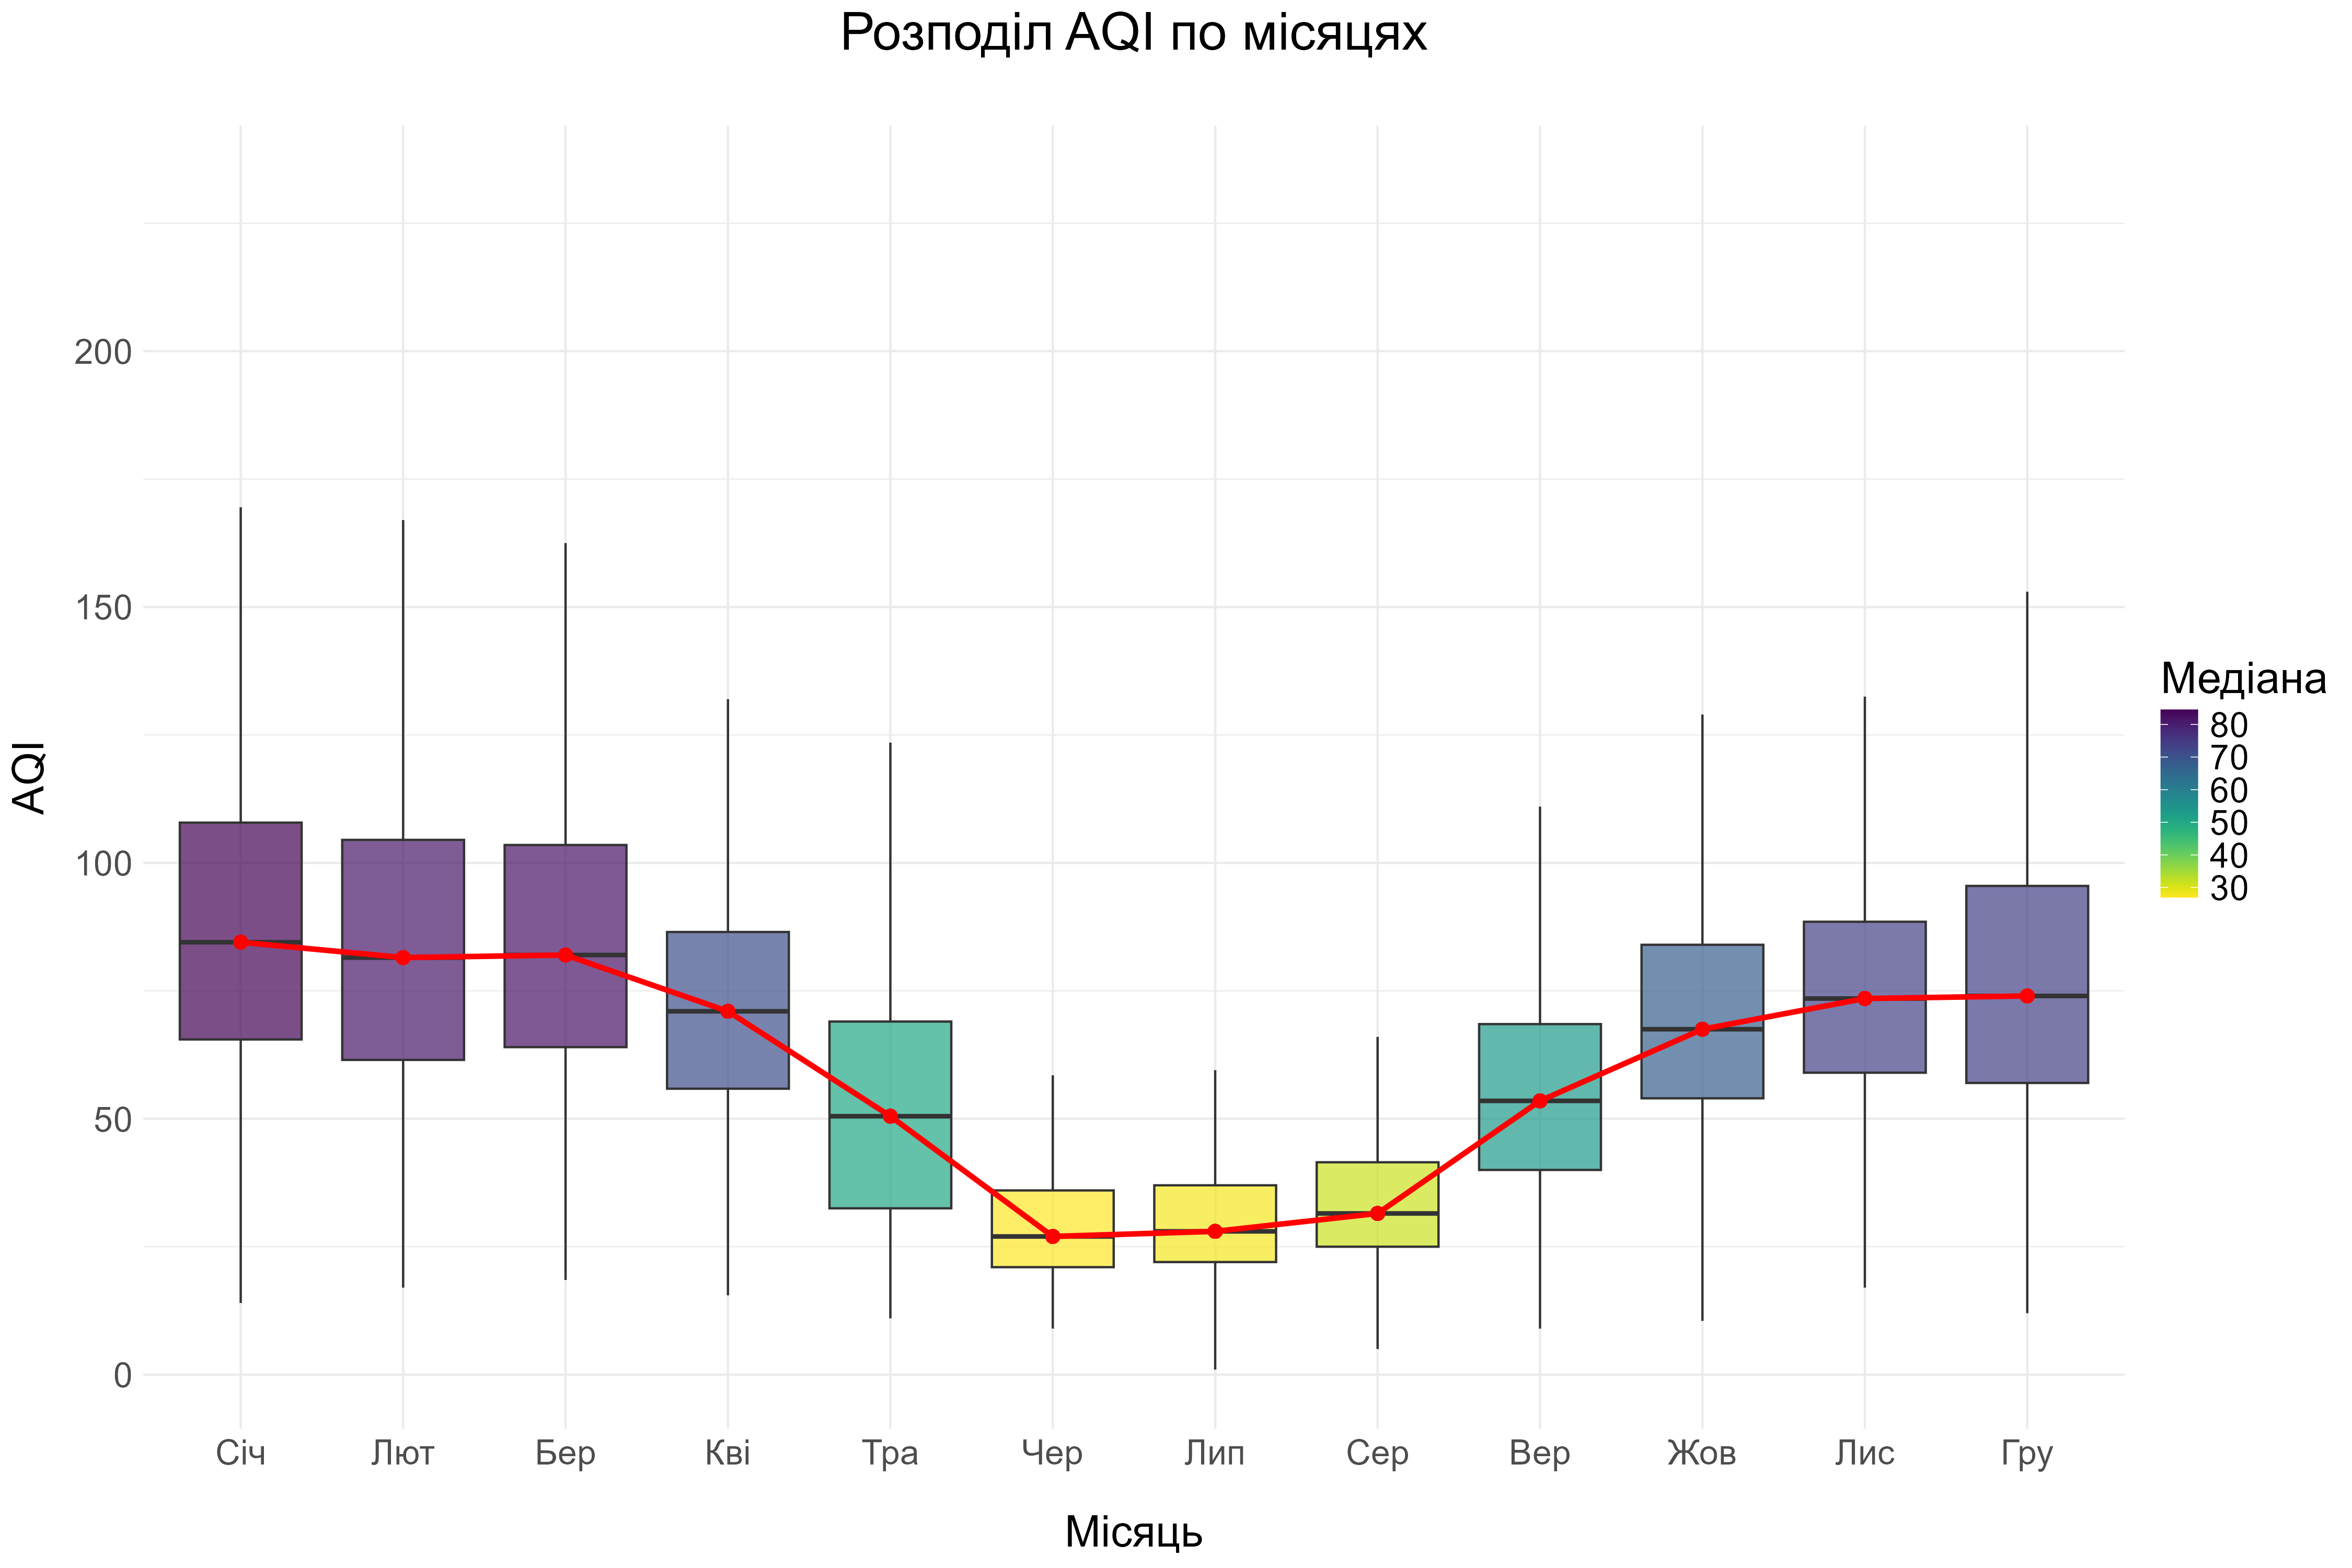
\includegraphics[height=2.8in]{plots/lab4/kernal/seasonal_change_median_line.png}
  \end{center}

  %Ядрова регресія — це непараметричний метод оцінки умовної математичної сподіваності залежної змінної $Y$ при заданому значенні незалежної змінної $X=x$.
  %\begin{itemize}
  %  \item \textbf{Оцінка Надарая-Вотсона (Nadaraya-Watson Estimator):}
  %  Найбільш поширена форма ядрової регресії. Оцінка функції регресії $m(x) = E[Y|X=x]$ в точці $x$ задається як:
  %  $$ \hat{m}_h(x) = \frac{\sum_{i=1}^{n} K_h(x - X_i) Y_i}{\sum_{i=1}^{n} K_h(x - X_i)} $$
  %  де:
  %  \begin{itemize}
  %      \item $n$ – кількість спостережень.
  %      \item $Y_i$ – значення залежної змінної для $i$-го спостереження.
  %      \item $X_i$ – значення незалежної змінної для $i$-го спостереження.
  %      \item $K_h(u) = \frac{1}{h}K(\frac{u}{h})$ – масштабоване ядро.
  %      \item $K(\cdot)$ – ядрова функція (kernel function).
  %      \item $h$ – параметр згладжування (bandwidth або ширина вікна).
  %  \end{itemize}
  %\end{itemize}
\end{frame}

%\begin{frame}
%  \frametitle{Ядрова регресія}
%  
%  \begin{center}
%    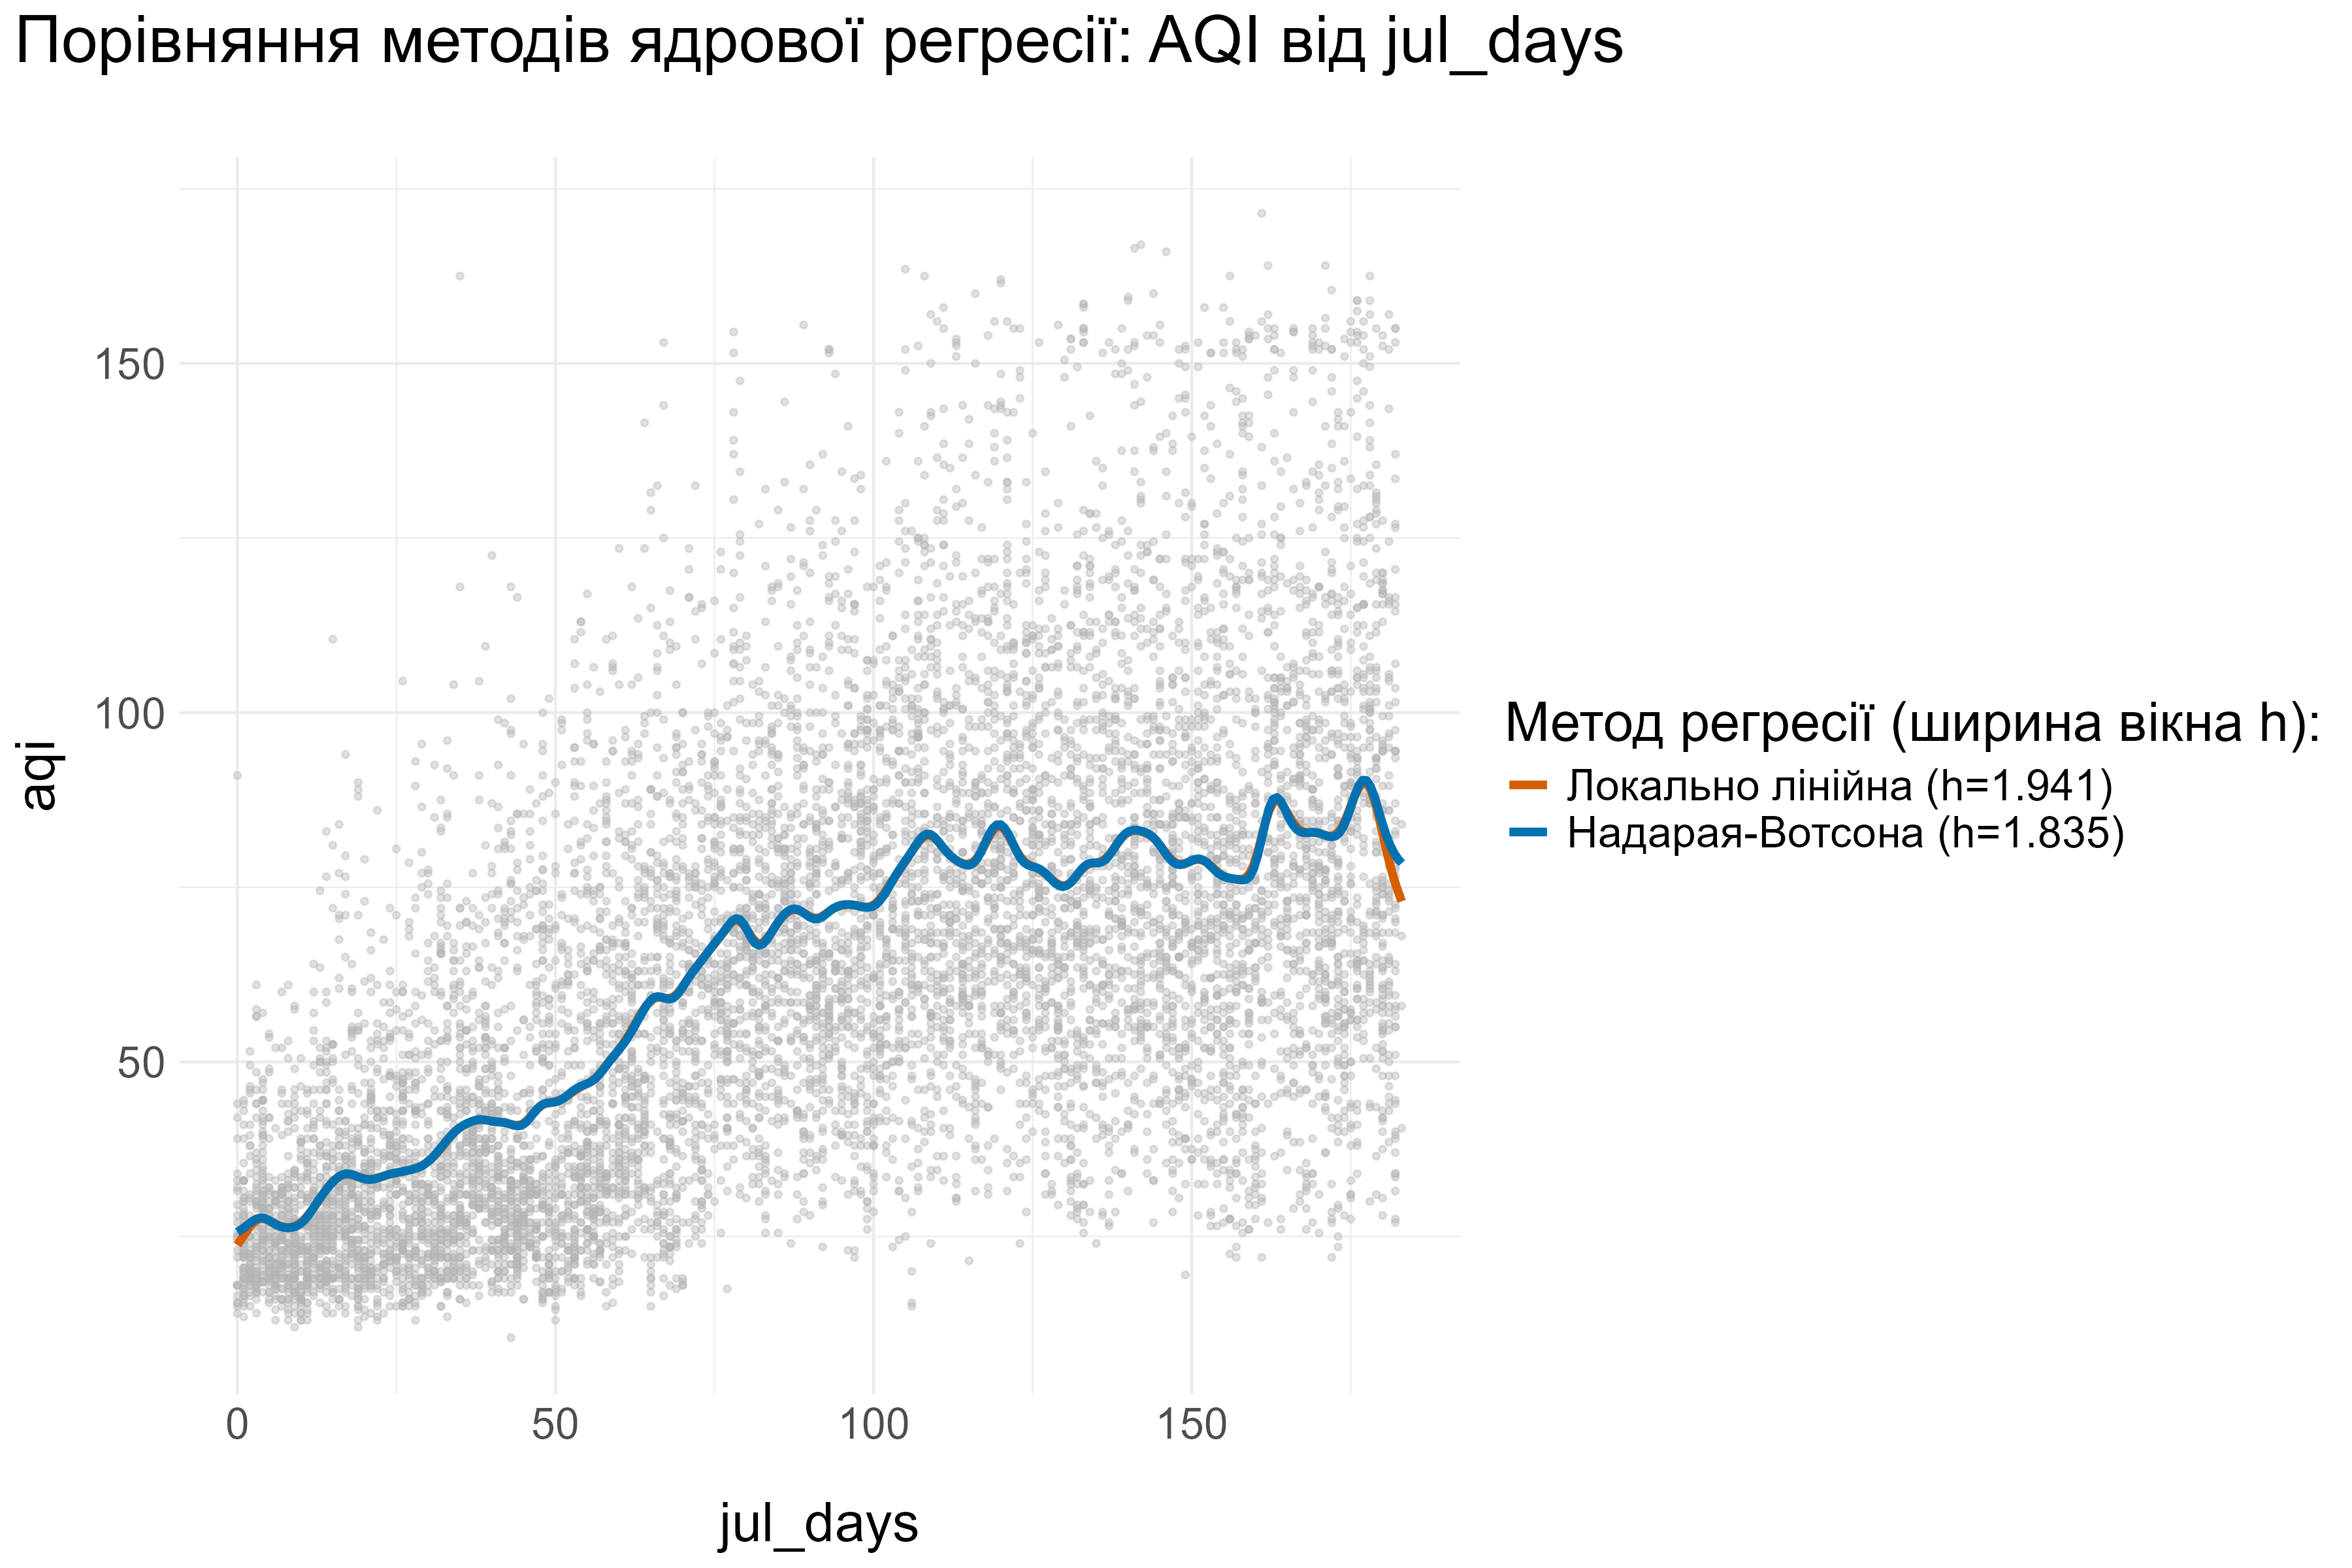
\includegraphics[height=2.8in]{plots/lab4/kernal/npreg_comparison_final_final.png}
%  \end{center}
% 
%  %\begin{itemize}
%  %  \item \textbf{Локальна поліноміальна регресія (Local Polynomial Regression):}
%  %  Узагальнення оцінки Надарая-Вотсона. Замість локального усереднення $Y_i$, вона апроксимує функцію регресії $m(x)$ локальним поліномом степеня $p$.
%  %  Для локально-лінійної регресії ($p=1$), оцінка $\hat{\beta}_0$ в точці $x$ є оцінкою $m(x)$:
%  %  $$ (\hat{\beta}_0, \hat{\beta}_1) = \arg\min_{\beta_0, \beta_1} \sum_{i=1}^{n} \left(Y_i - \beta_0 - \beta_1(X_i - x)\right)^2 K_h(X_i - x) $$
%  %  Тоді $\hat{m}_h(x) = \hat{\beta}_0$.
%  %  Локальні поліноми вищих порядків можуть краще адаптуватися до кривизни функції та зменшувати зміщення на границях.
%  %\end{itemize}
%\end{frame}

\begin{frame}
  \frametitle{Ядрова регресія}
  
  \begin{center}
    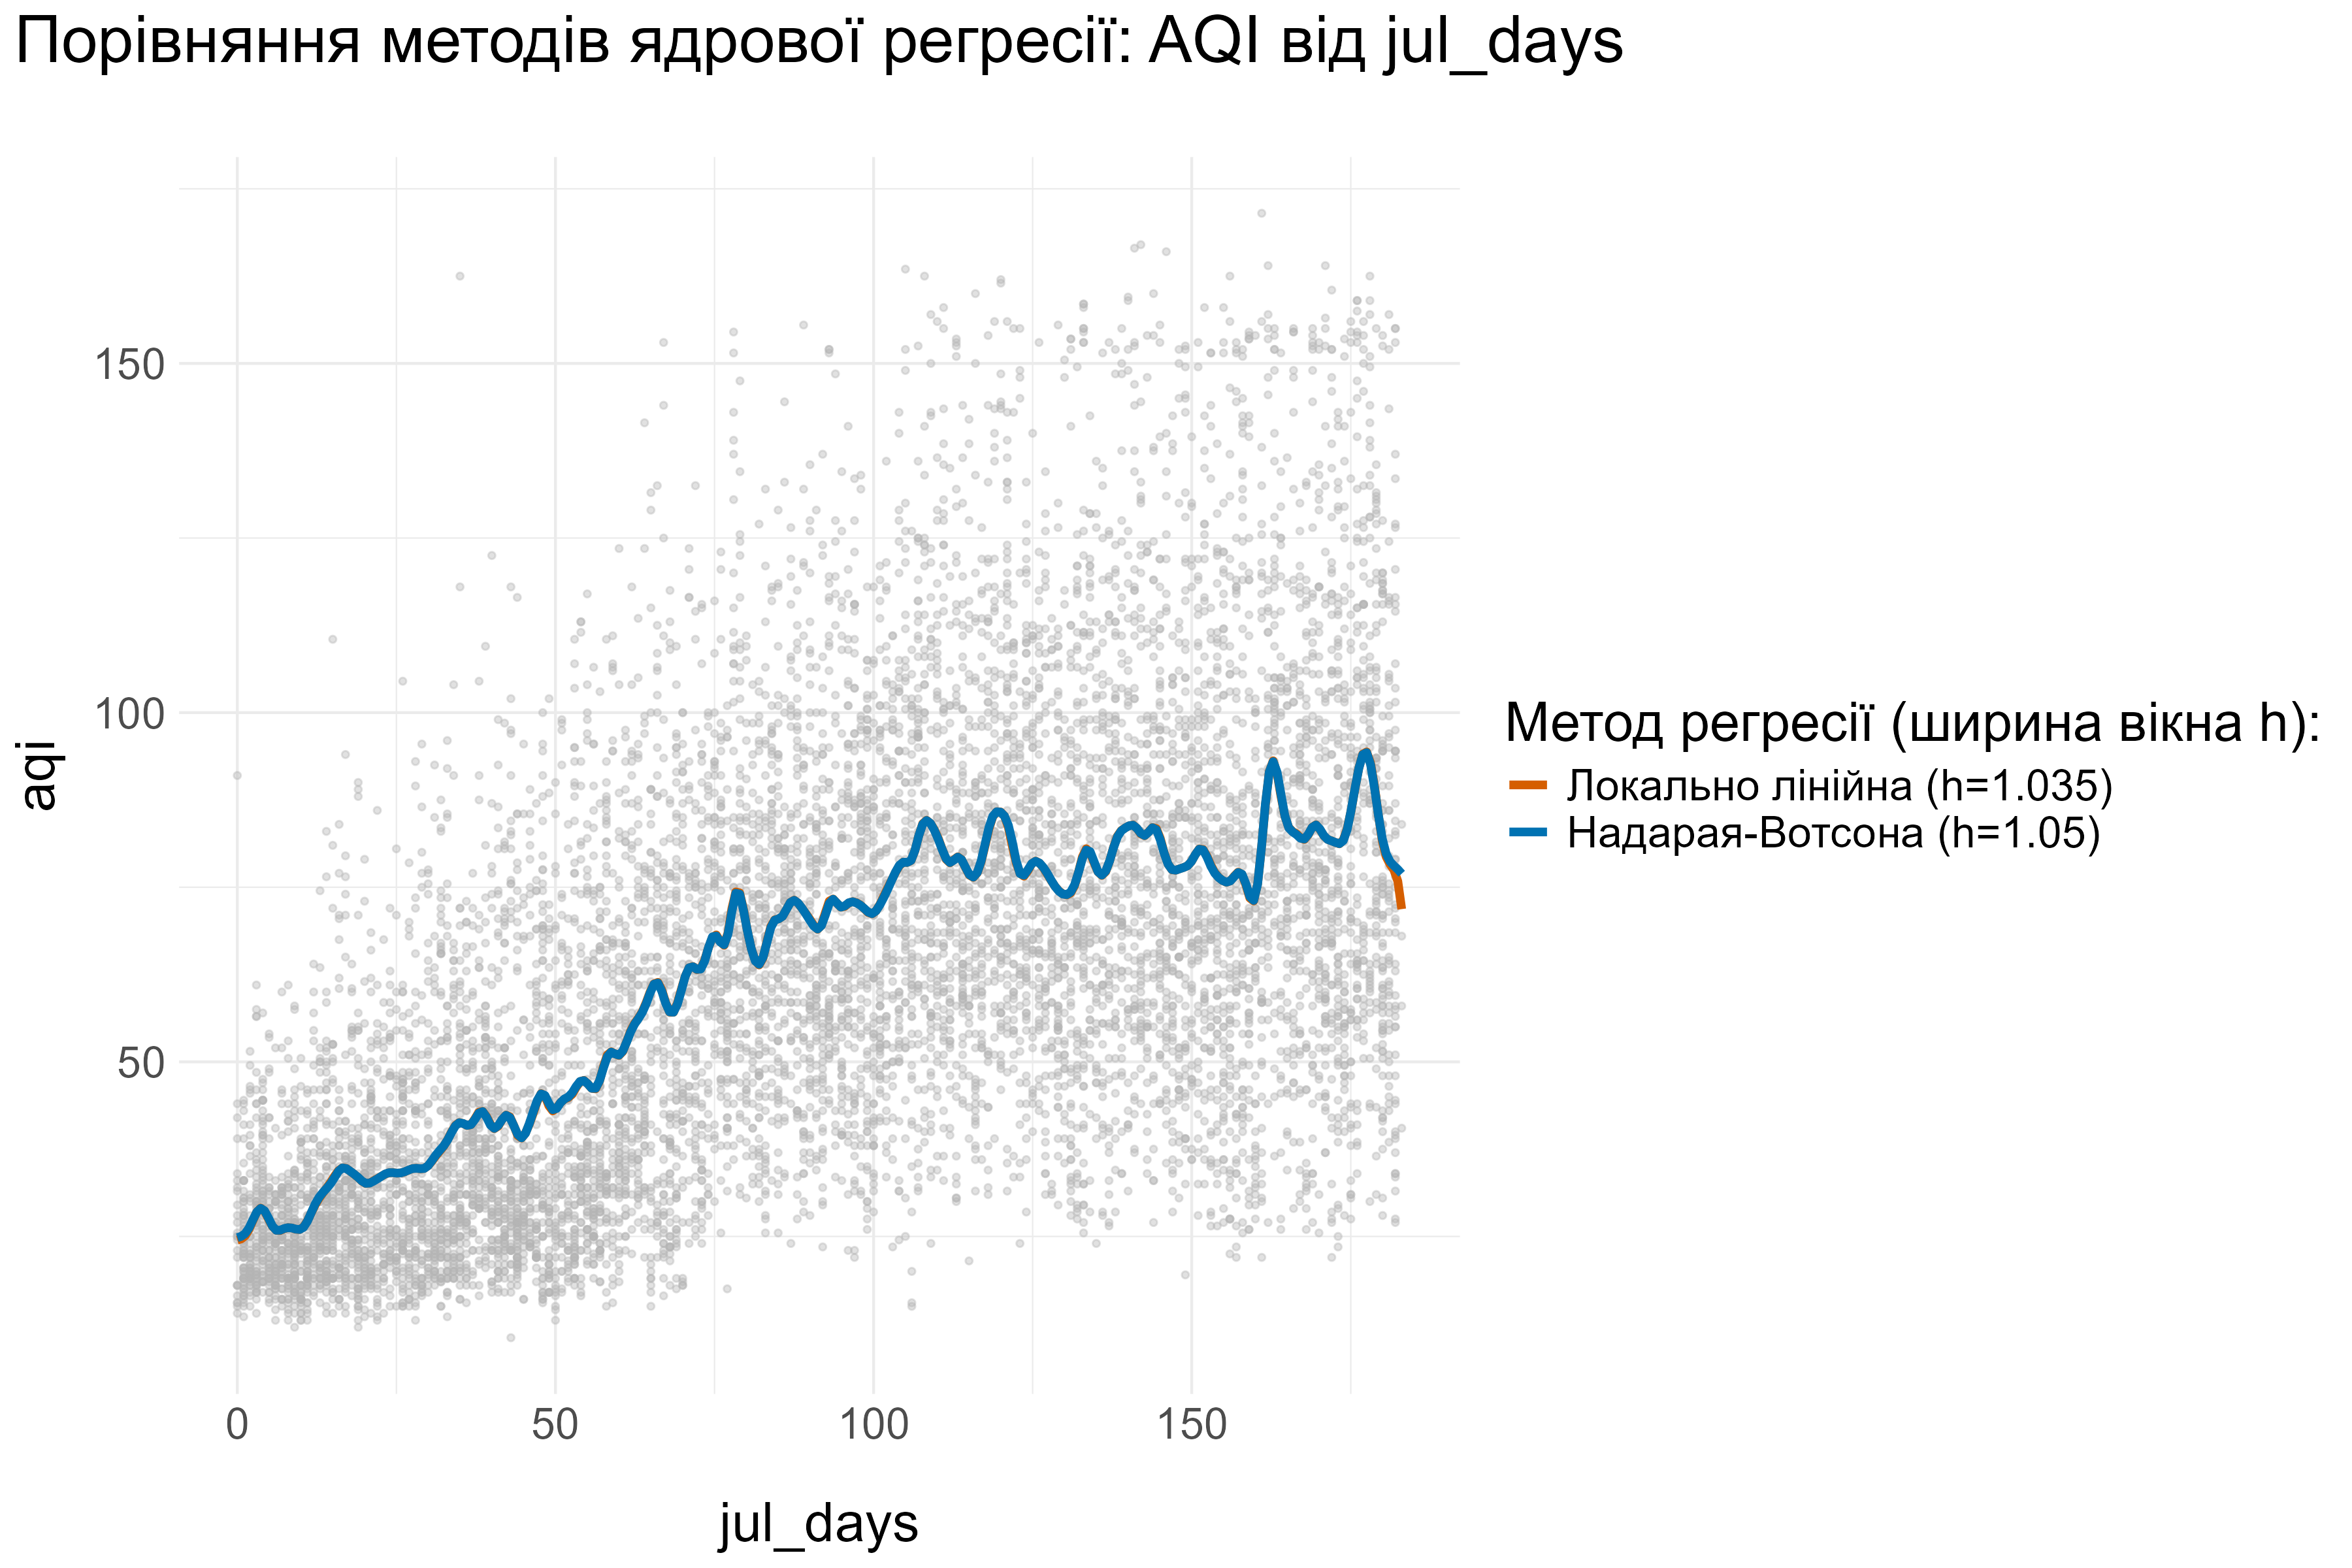
\includegraphics[height=2.8in]{plots/lab4/kernal/npreg_comparison_final_10.png}
  \end{center}
 
\end{frame}

\begin{frame}
  \frametitle{Ядрова регресія}
  
  \begin{center}
    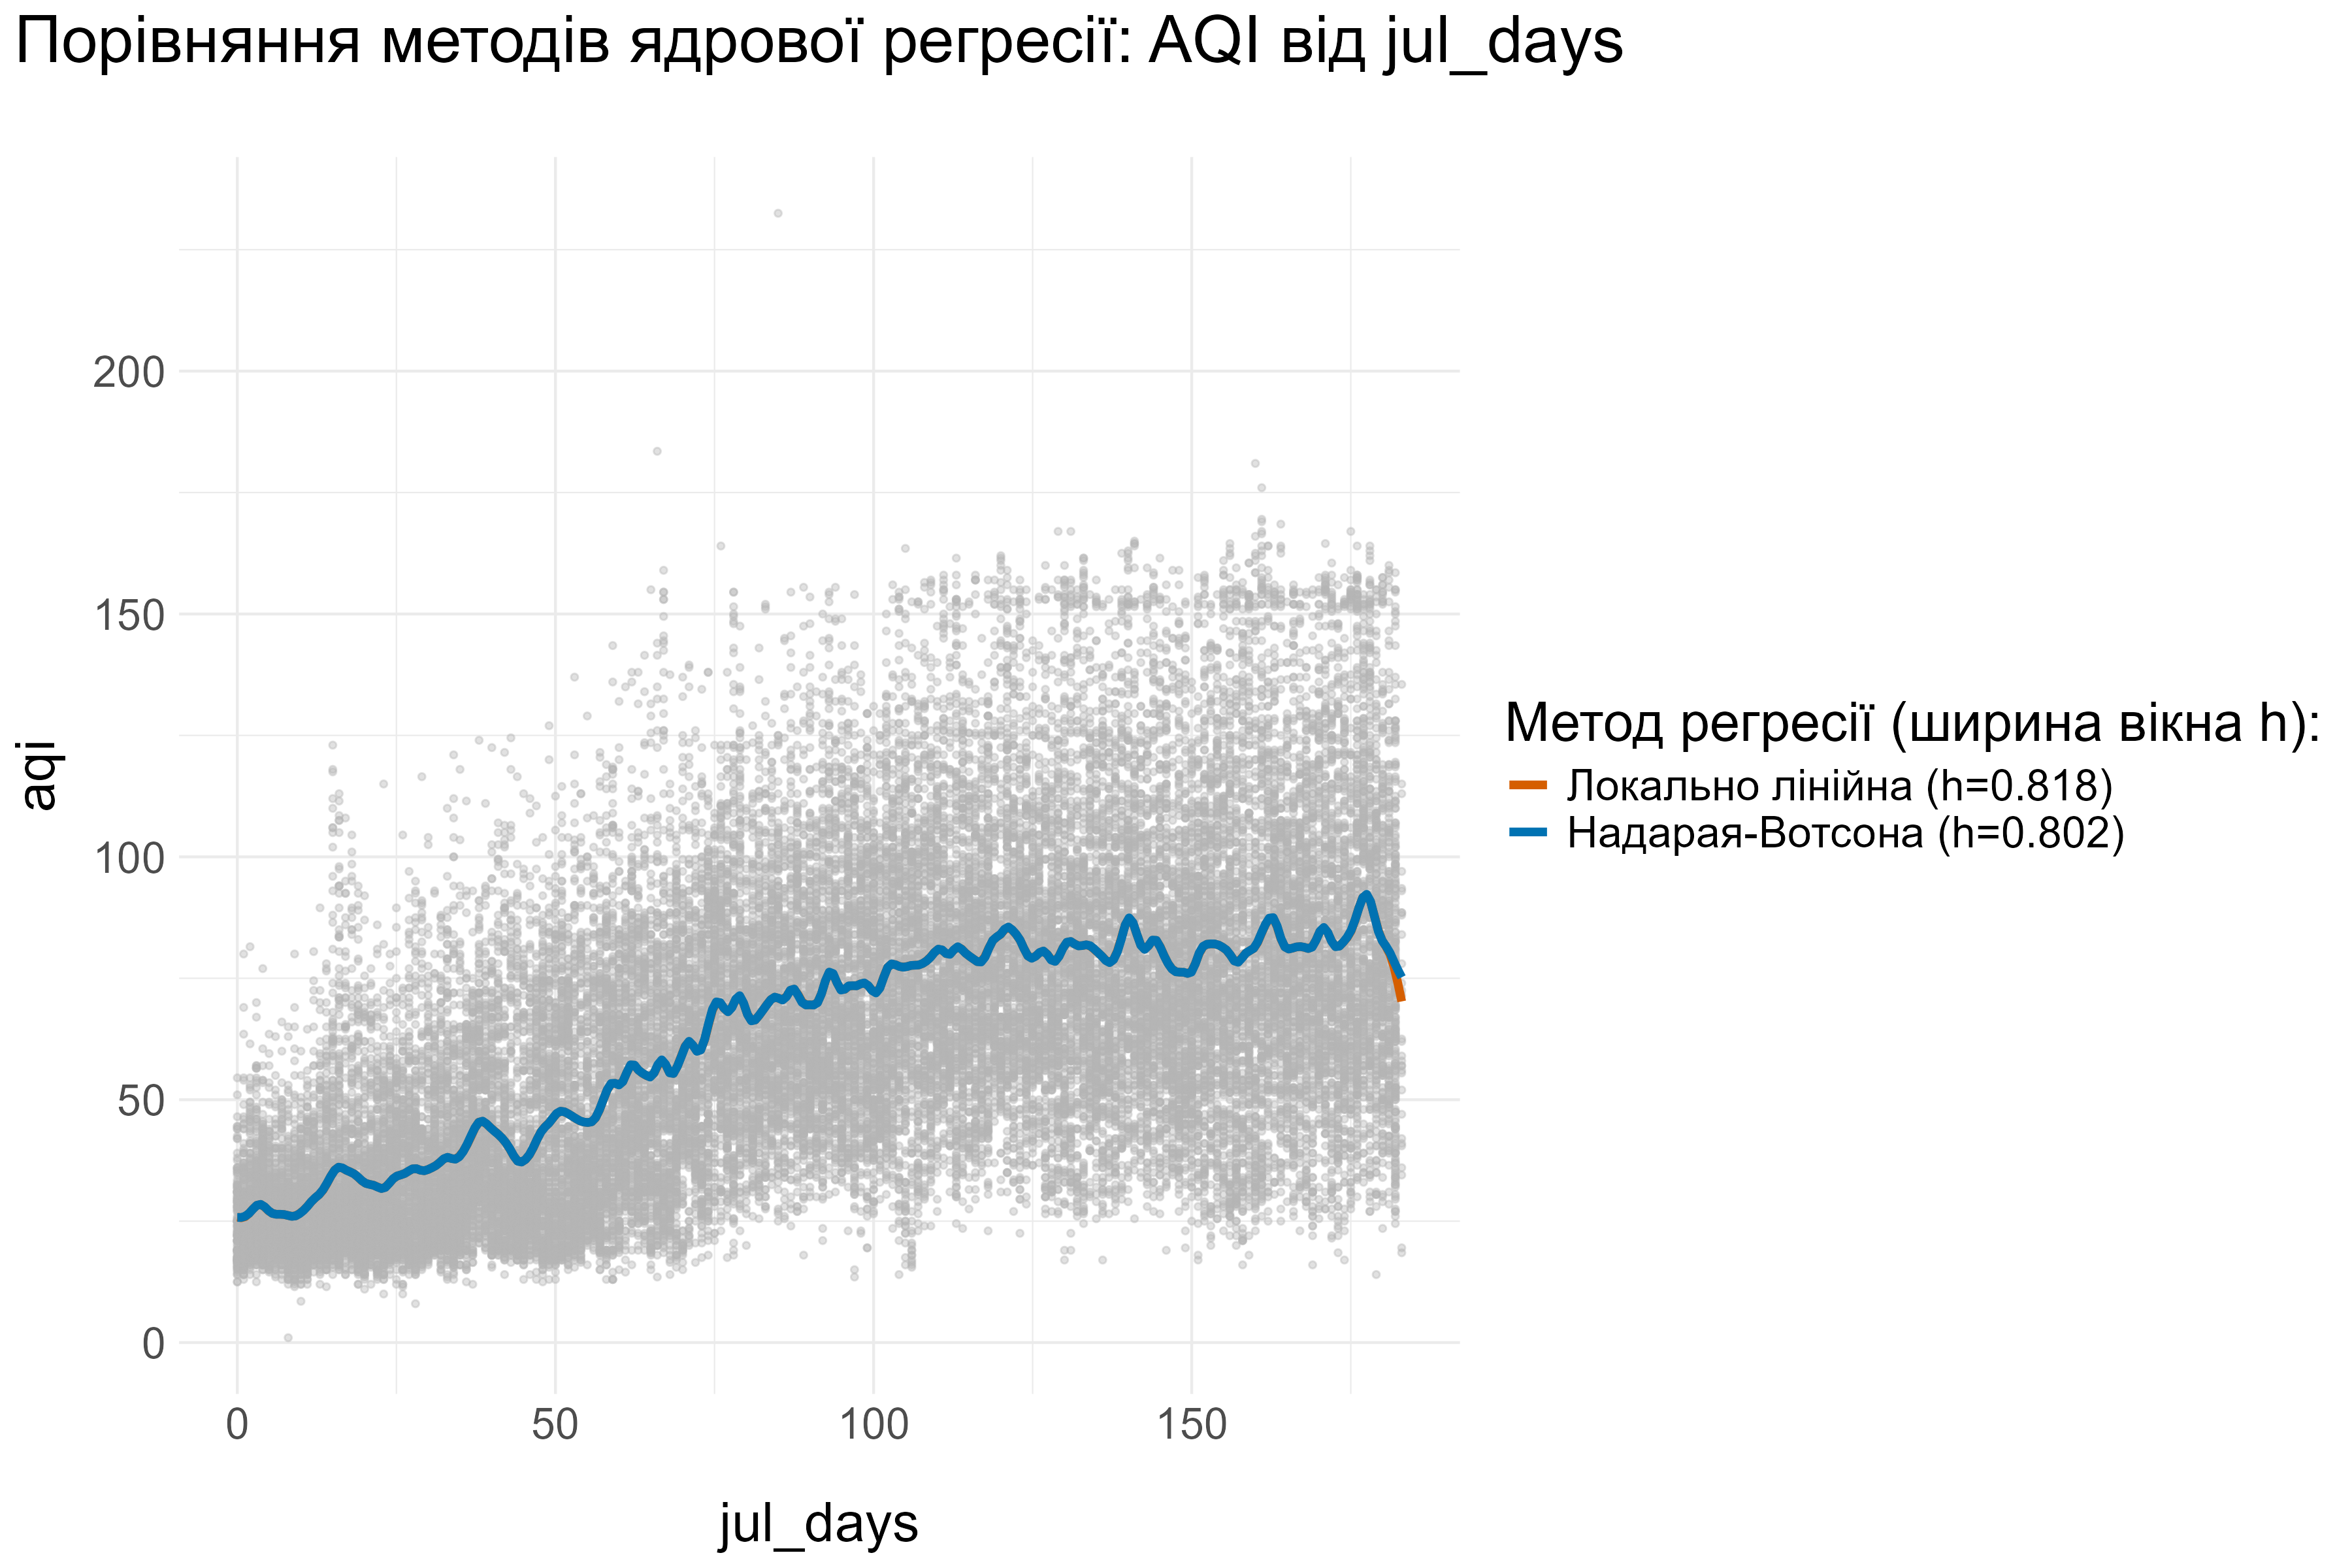
\includegraphics[height=2.8in]{plots/lab4/kernal/npreg_comparison_final_40.png}
  \end{center}
 
\end{frame}

\begin{frame}
  \frametitle{Оцінка моделі}
  \resizebox{\textwidth}{!}{%
    \begin{tabular}{l l r r r r r}
      \toprule
      Розмір вибірки & Метод & Bandwidth (h) & $R^2$ & RMSE (навч.) & RMSE (тест) & MAE (тест) \\
      \midrule 
      10 тис. & Надарая-Вотсона & 1.0499 & 0.4094 & 24.369 & 24.706 & 19.112 \\
      10 тис. & Локально лінійна & 1.0346 & 0.4096 & 24.364 & 24.709 & 19.117 \\
      \midrule
      40 тис. & Надарая-Вотсона  & 0.8020 & 0.4069 & 24.561 & 24.464 & 18.861\\
      40 тис. & Локально лінійна  & 0.8184 & 0.4068 & 24.562 & 24.463 & 18.858\\
      \bottomrule
    \end{tabular}%
  }
\end{frame}

\begin{frame}
  \frametitle{Підсумок моделі}
  \begin{columns}[T] 
  \begin{column}{0.48\textwidth} 
  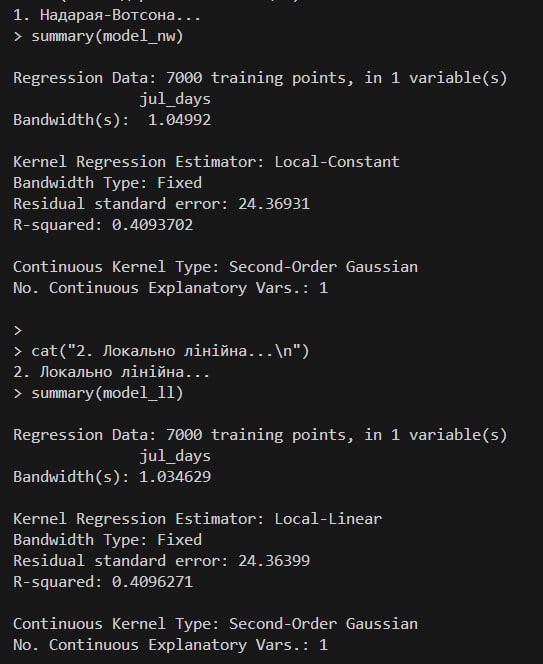
\includegraphics[width=\textwidth]{plots/lab4/kernal/10.jpg}
  \captionof{figure}{Summary 10 тисяч}
  \end{column}
  \hfill
  \begin{column}{0.48\textwidth} 
  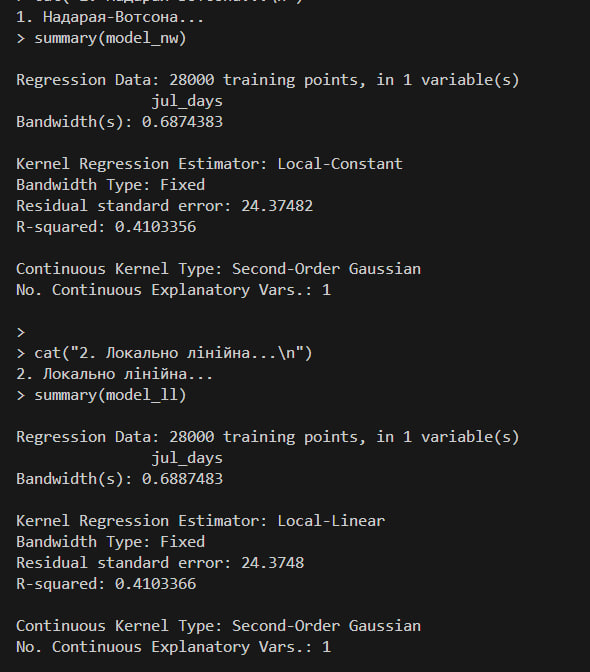
\includegraphics[width=\textwidth]{plots/lab4/kernal/40.jpg}
  \captionof{figure}{Summary 40 тисяч}
  \end{column}
  \end{columns}
 
\end{frame}


\begin{frame}
  \frametitle{Висновок}
  \begin{itemize}
    \item Обидві моделі показали майже однакову якість за всіма метриками. 
    \item $ R^2 = 0.41 $ вказує на те, що моделі мають обмежену здатність пояснювати варіацію у даних.
    \item Вибір між ними може залежати не стільки від якості, скільки від стійкості до шуму чи переваг у теоретичних властивостях.
  \end{itemize}
\end{frame}


\begin{frame}
  \section{Частково-лінійна модель}

  \frametitle{Зміст}
  \tableofcontents[currentsection]
\end{frame}

\begin{frame}
  \frametitle{Розподіл регресорів}
  
  Непараметричні:
  
  \begin{itemize}
    \item \texttt{jul\_days}: кількість днів до найближчого 1-го липня.
  \end{itemize}
  
  Параметричні:
  \begin{itemize}
    \item \texttt{reform\_days}: кількість днів з початку реформи.
    \item \texttt{windspeed}: швидкість вітру в м/с.
    \item \texttt{county}\footnotemark: регіон, у якому проводилося вимірювання.
  \end{itemize}
  
  \footnotetext[1]{Відсутня в моделі 2.1, наявна в моделі 2.2}

\end{frame}

\begin{frame}
  \frametitle{Оцінка регресорів}

  \begin{table}
  \centering
  \begin{talltblr}[         %% tabularray outer open
  entry=none,label=none,
  note{}={+ p \num{< 0.1}, * p \num{< 0.05}, ** p \num{< 0.01}, *** p \num{< 0.001}},
  ]                     %% tabularray outer close
  {                     %% tabularray inner open
  colspec={Q[]Q[]Q[]},
  column{2,3}={}{halign=c,},
  column{1}={}{halign=l,},
  hline{22}={1,2,3}{solid, black, 0.05em},
  }                     %% tabularray inner close
  \toprule
  & nppl (2.1) & nppl (2.2) \\ \midrule %% TinyTableHeader
  reform\_days & \num{-0.009989}*** & \num{-0.010092}*** \\
  & (\num{0.000342}) & (\num{0.000342}) \\
  windspeed & \num{-2.758367}*** & \num{-3.229516}*** \\
  & (\num{0.255418}) & (\num{0.281014}) \\ \midrule
  Num.Obs. & 7000 & 7000 \\
  R2 & 0.479709 & 0.485264 \\
  RMSE & 23.287205 & 23.110408 \\
  \bottomrule
  \end{talltblr}
  \end{table} 
\end{frame}

\begin{frame}
  \frametitle{Оцінка регресорів}
  
  \begin{ssmall}
  
  \begin{table}
  \centering
  \begin{talltblr}[         %% tabularray outer open
  entry=none,label=none,
  note{}={+ p \num{< 0.1}, * p \num{< 0.05}, ** p \num{< 0.01}, *** p \num{< 0.001}},
  ]                     %% tabularray outer close
  {                     %% tabularray inner open
  colspec={Q[]Q[]Q[]},
  column{2,3}={}{halign=c,},
  column{1}={}{halign=l,},
  hline{22}={1,2,3}{solid, black, 0.05em},
  }                     %% tabularray inner close
  \toprule
  & nppl (2.1) & nppl (2.2) \\ \midrule %% TinyTableHeader
  Kaohsiung\_City &  & \num{7.409501} \\
  &  & (\num{61.460824}) \\
  Chiayi\_City &  & \num{4.498697} \\
  &  & (\num{61.470944}) \\
  Kinmen\_County &  & \num{10.172092} \\
  &  & (\num{61.484341}) \\
  Lienchiang\_County &  & \num{4.879358} \\
  &  & (\num{61.496276}) \\
  Chiayi\_County &  & \num{4.051747} \\
  &  & (\num{61.465913}) \\
  Yunlin\_County &  & \num{7.979392} \\
  &  & (\num{61.464152}) \\
  Tainan\_City &  & \num{4.716426} \\
  &  & (\num{61.471446}) \\
  Nantou\_County &  & \num{0.239960} \\
  &  & (\num{61.458835}) \\
  \bottomrule
  \end{talltblr}
  \end{table} 
  
  \end{ssmall}
\end{frame}

\begin{frame}
  \frametitle{Оцінка регресорів}

   \begin{center}
    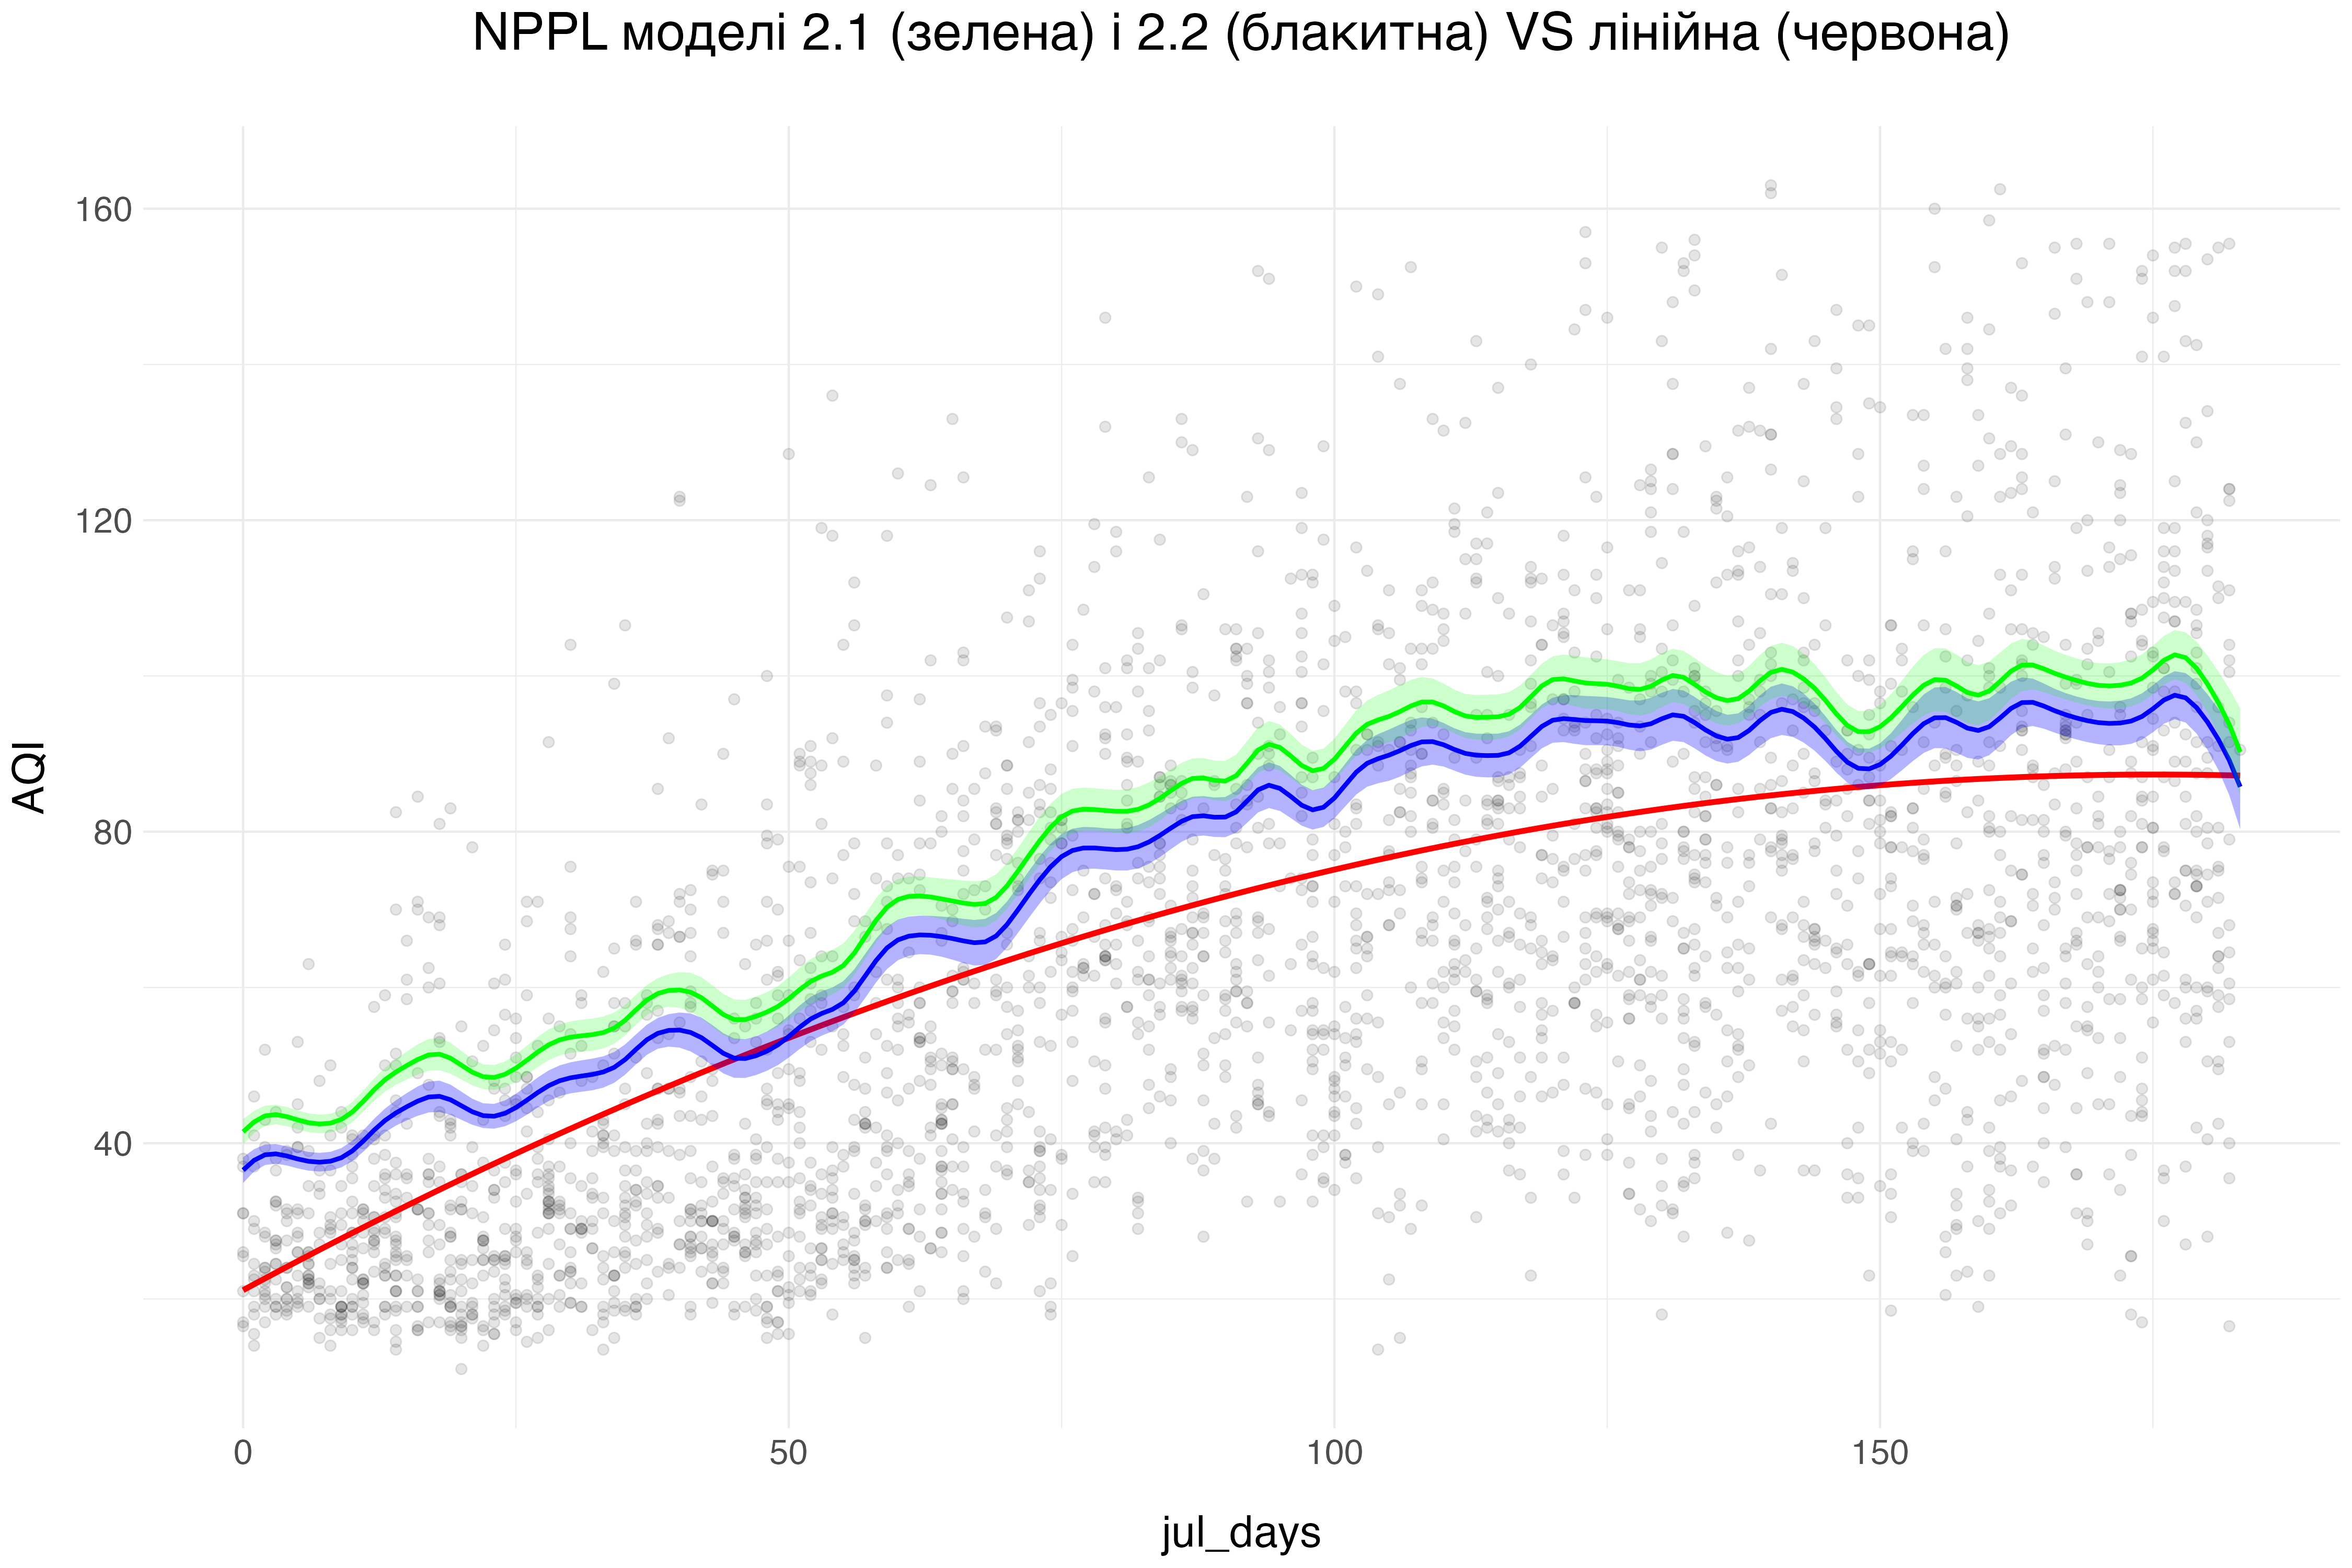
\includegraphics[height=2.8in]{plots/lab4/partial_linear/nppl_vs_lin.png}
  \end{center}
\end{frame}

\begin{frame}
  \frametitle{Регресор after\_reform замість reform\_days}
  
  \begin{table}
  \centering
  \begin{talltblr}[         %% tabularray outer open
  entry=none,label=none,
  note{}={+ p \num{< 0.1}, * p \num{< 0.05}, ** p \num{< 0.01}, *** p \num{< 0.001}},
  ]                     %% tabularray outer close
  {                     %% tabularray inner open
  colspec={Q[]Q[]},
  column{2}={}{halign=c,},
  column{1}={}{halign=l,},
  hline{6}={1,2}{solid, black, 0.05em},
  }                     %% tabularray inner close
  \toprule
  & nppl (3) \\ \midrule %% TinyTableHeader
  after\_reform & \num{-17.638269}*** \\
  & (\num{0.631408}) \\
  windspeed & \num{-3.195055}*** \\
  & (\num{0.254649}) \\
  Num.Obs. & 7000 \\
  R2 & 0.5449 \\
  RMSE & 25.503944 \\
  \bottomrule
  \end{talltblr}
  \end{table} 
\end{frame}

\begin{frame}
\frametitle{Регресор after\_reform замість reform\_days}
  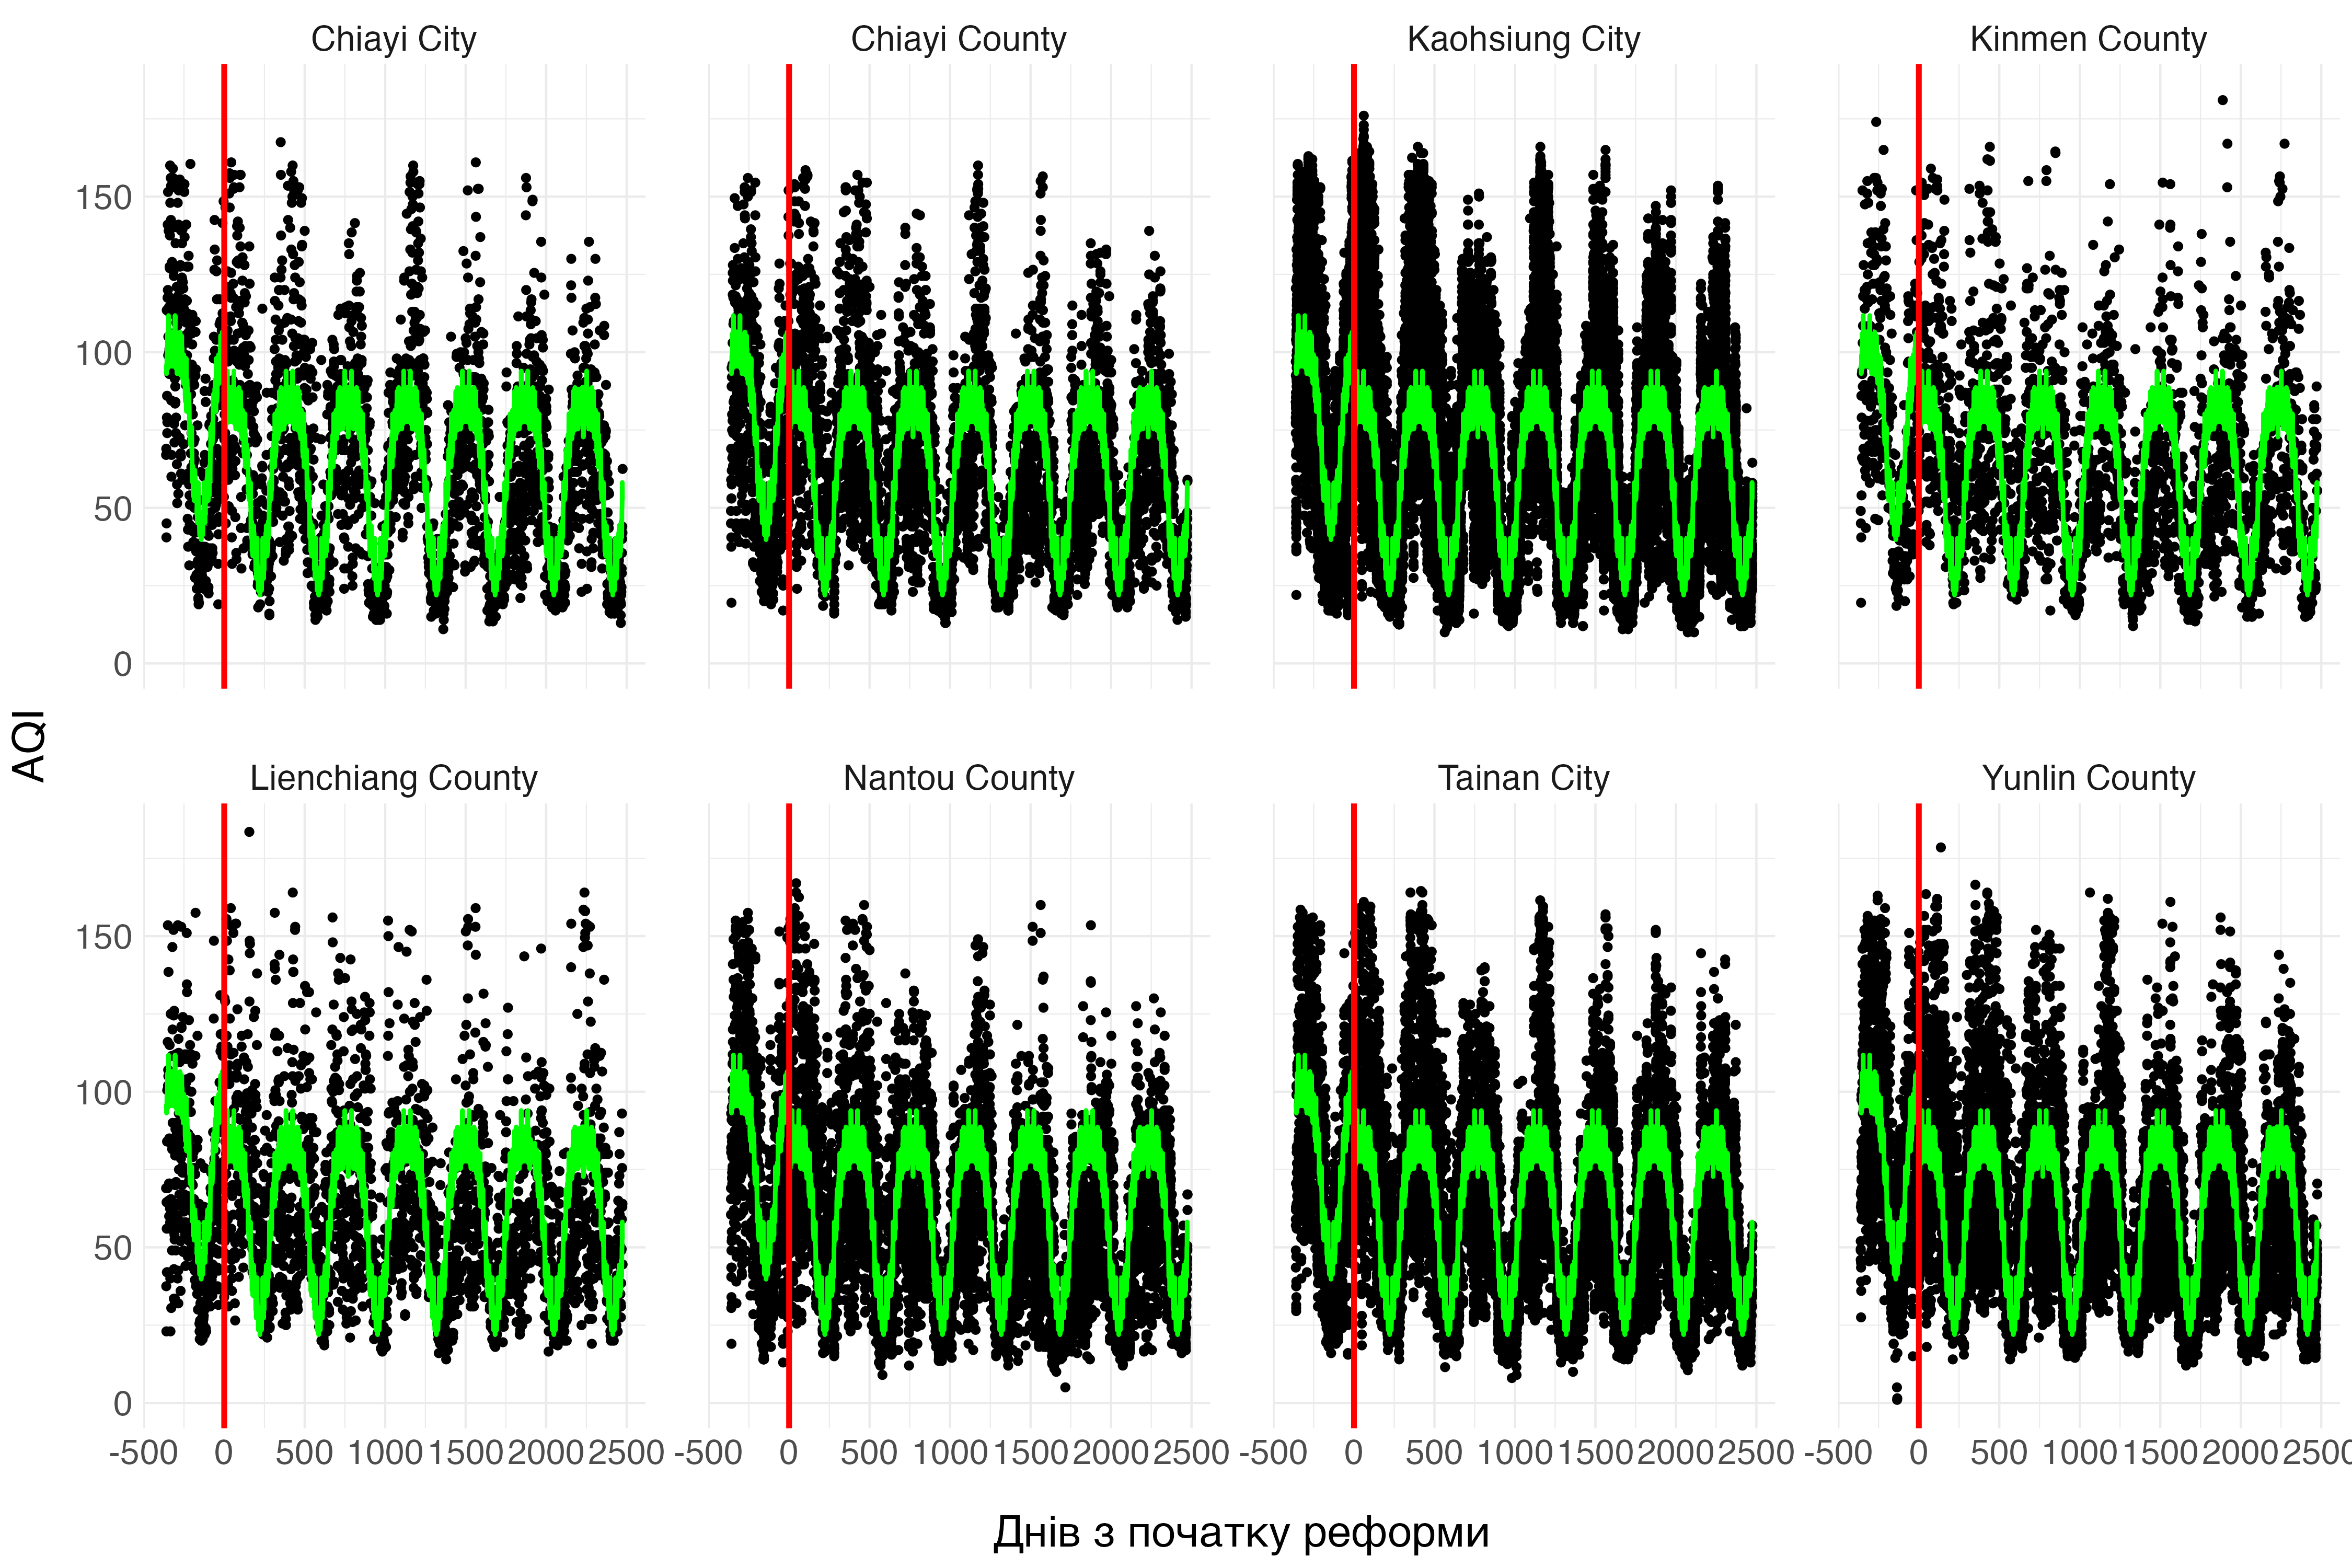
\includegraphics[height=2.8in]{plots/lab4/partial_linear/nppl_w_after_reform.png}
\end{frame}

\begin{frame}
  \section{Аналіз головних компонент}

  \frametitle{Зміст}
  \tableofcontents[currentsection]
\end{frame}

\begin{frame}
\frametitle{Аналіз головних компонент(Scree plot)}
  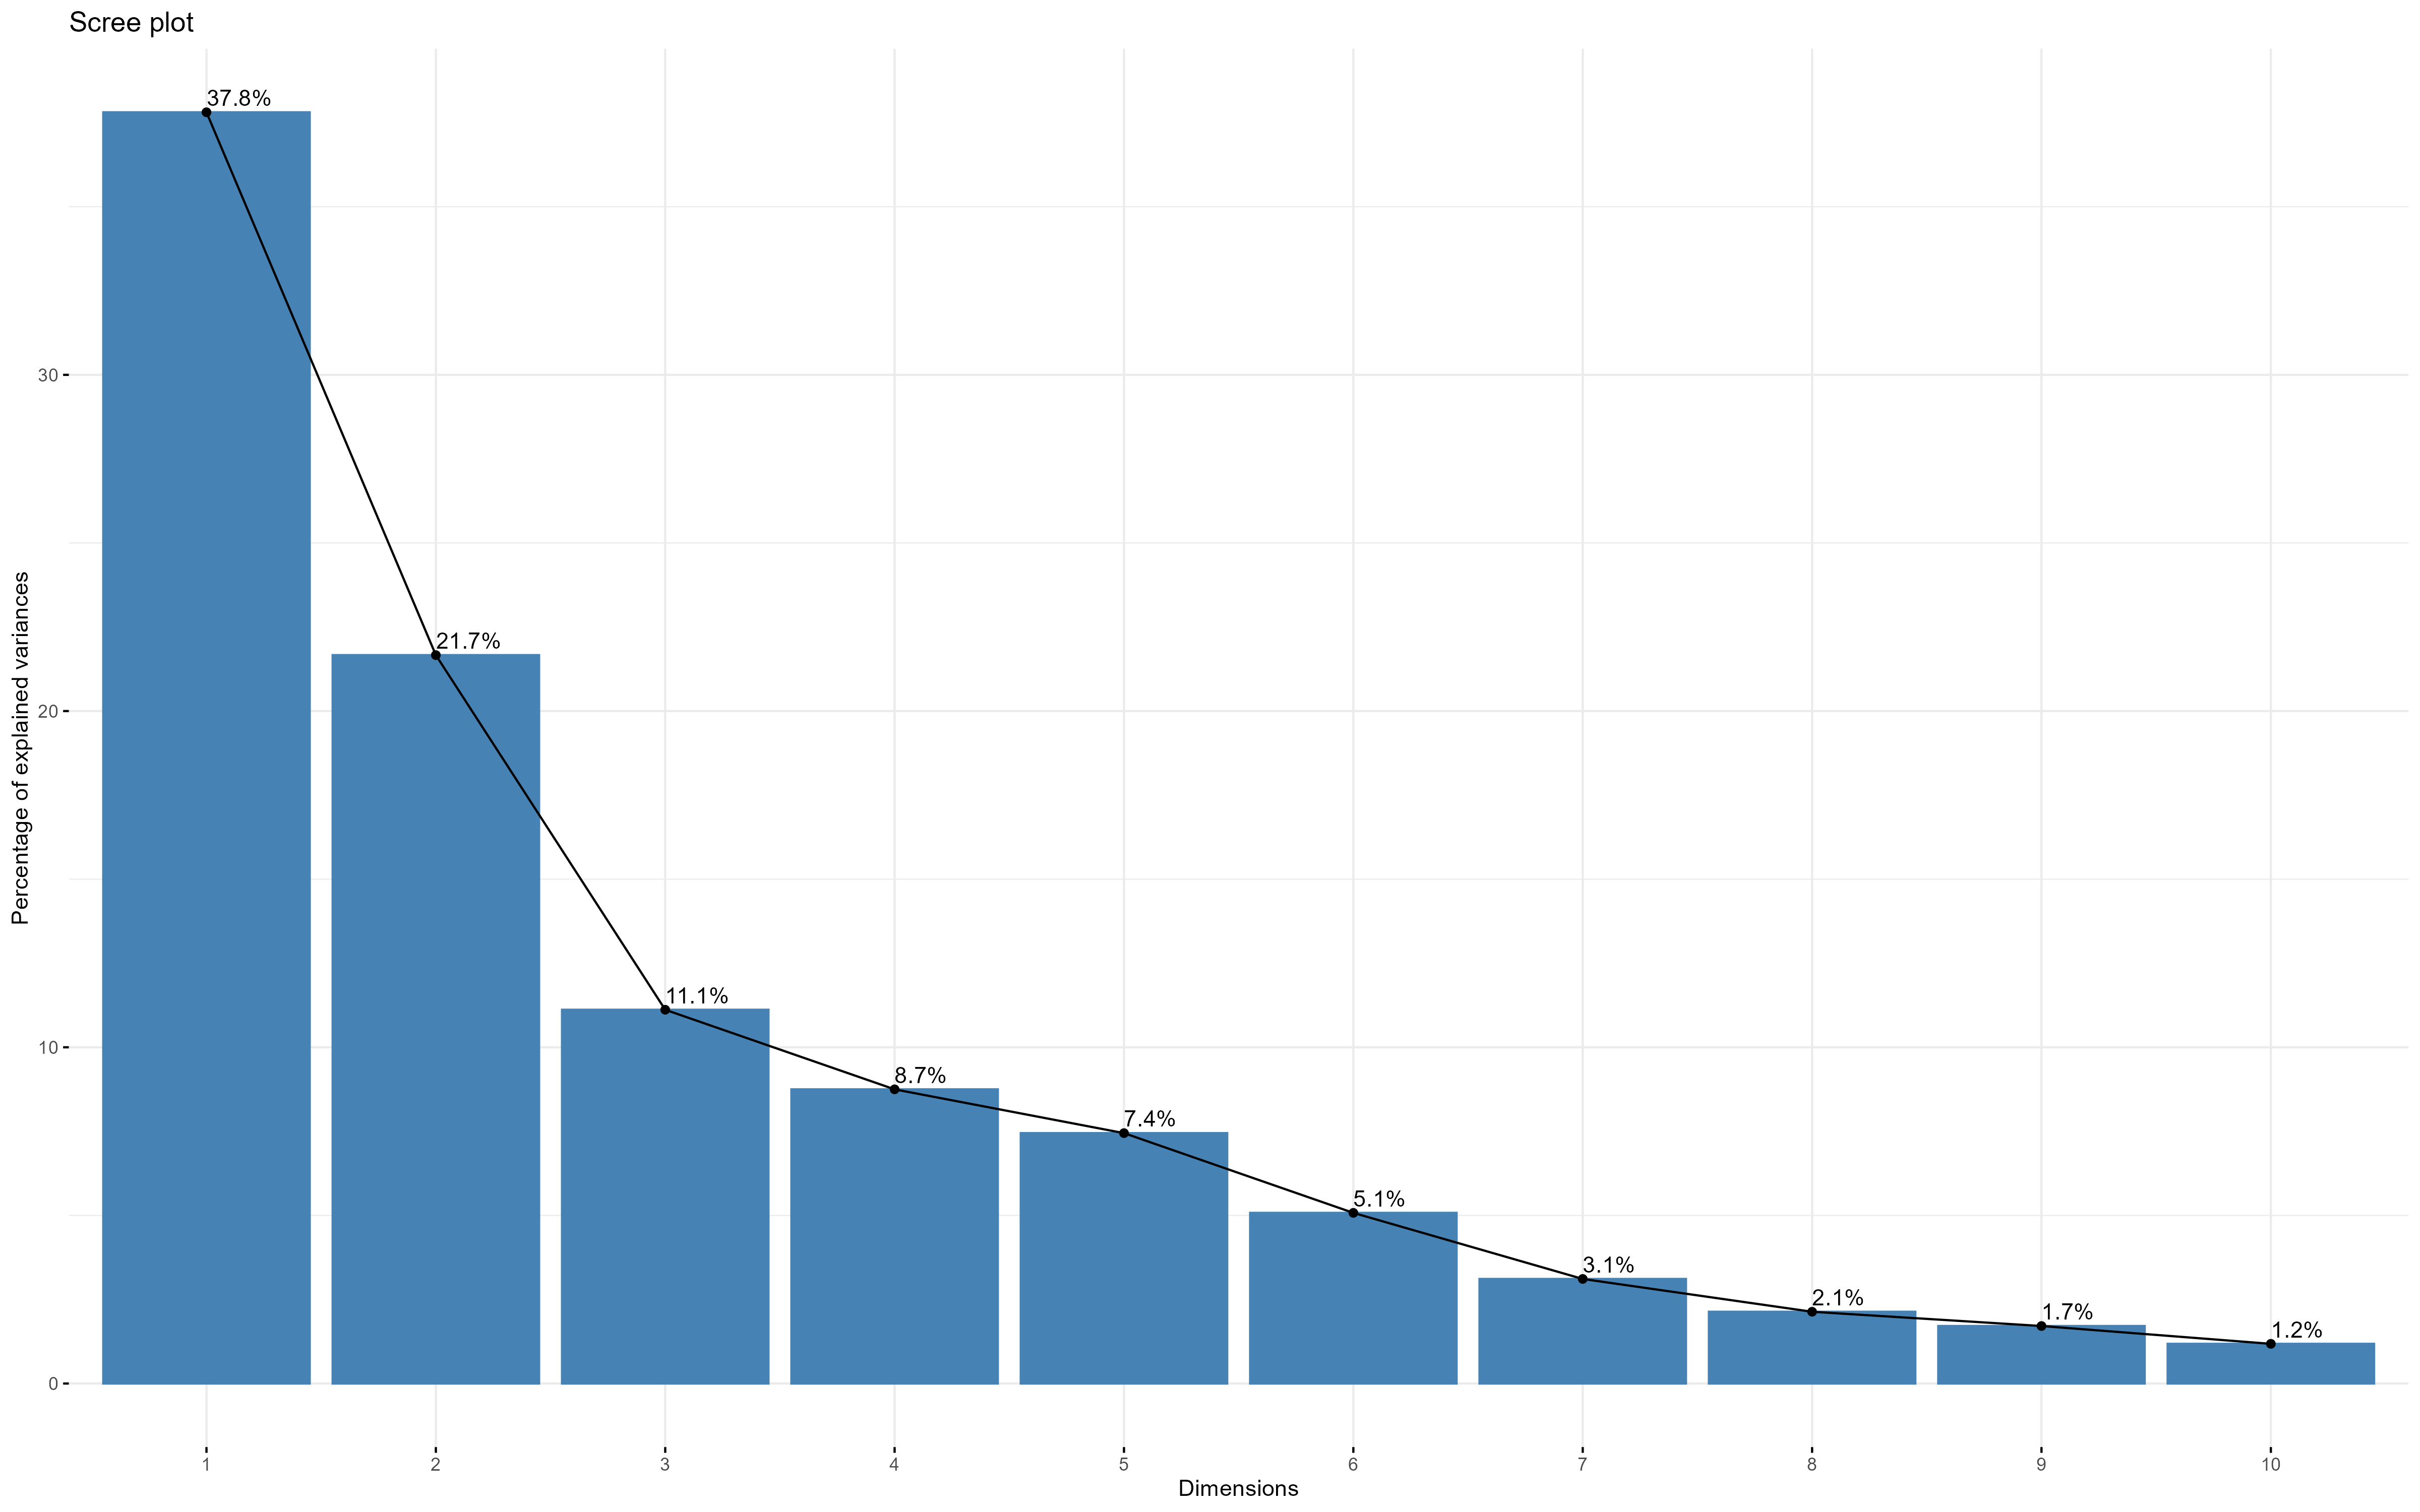
\includegraphics[height=2.8in]{plots/lab4/pca/scree.png}
\end{frame}

\begin{frame}
\frametitle{Аналіз головних компонент(Projection-1)}
  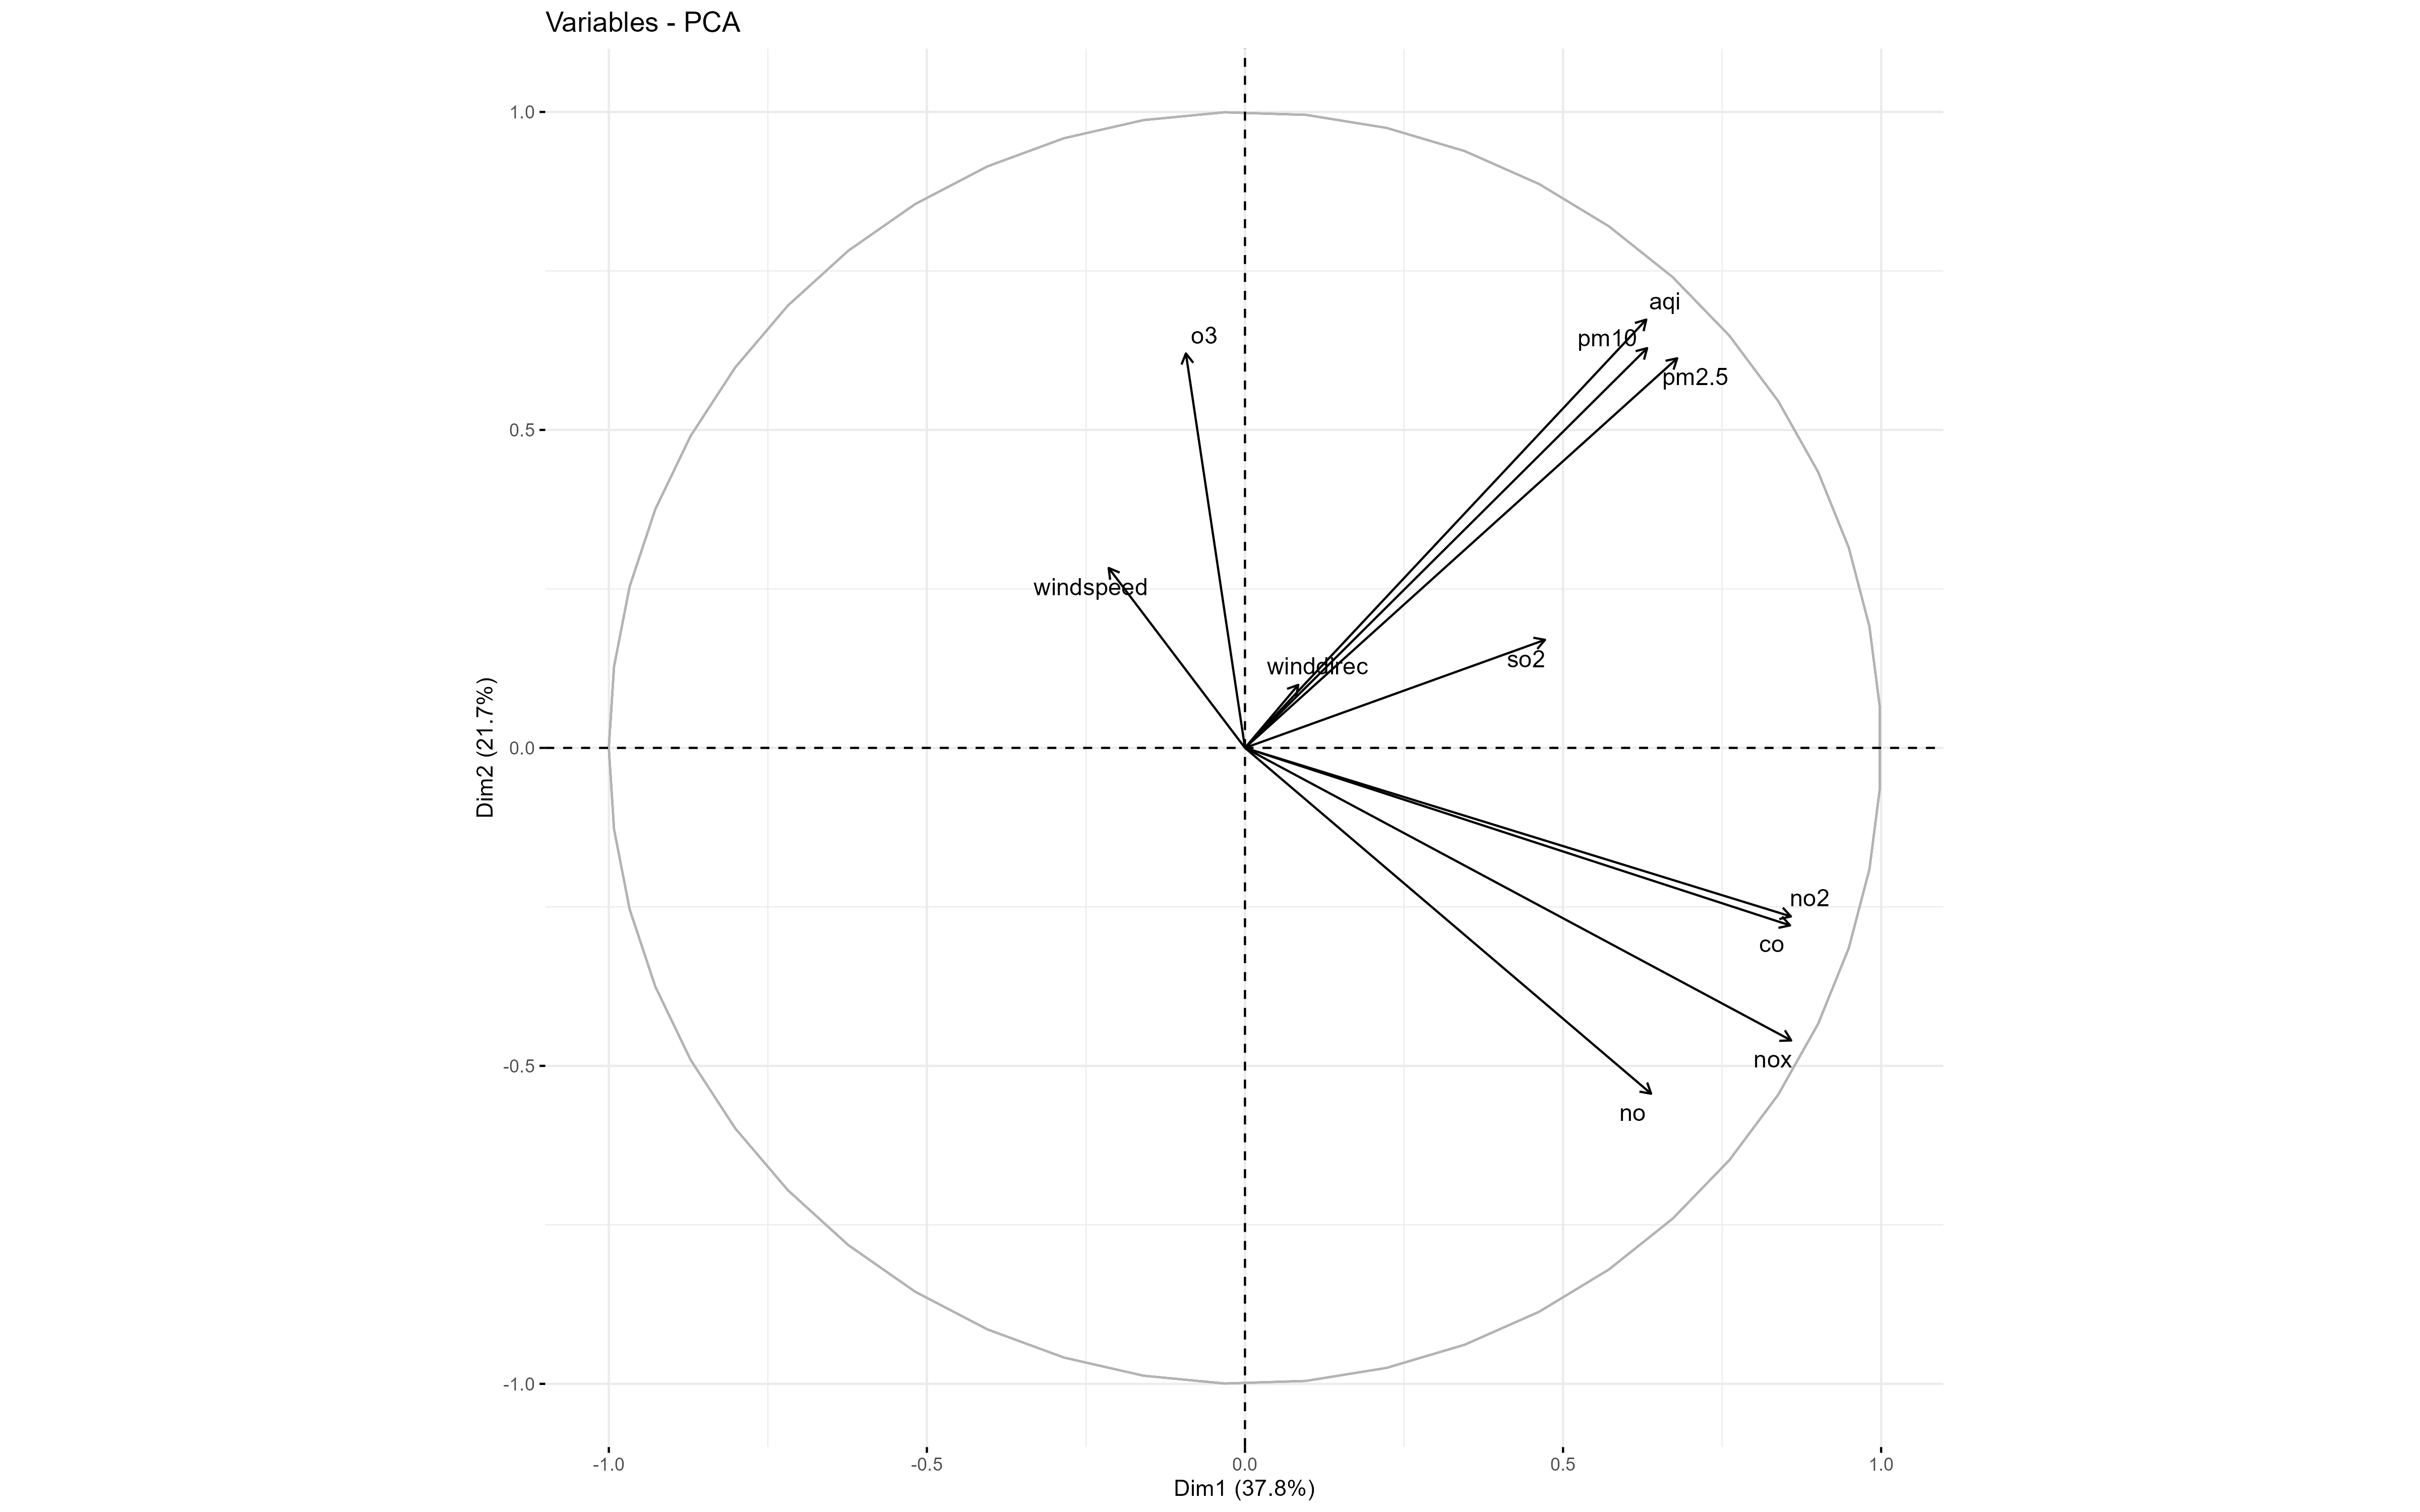
\includegraphics[height=2.8in]{plots/lab4/pca/projection-1-2.png}
\end{frame}

\begin{frame}
\frametitle{Аналіз головних компонент(Projection-2)}
  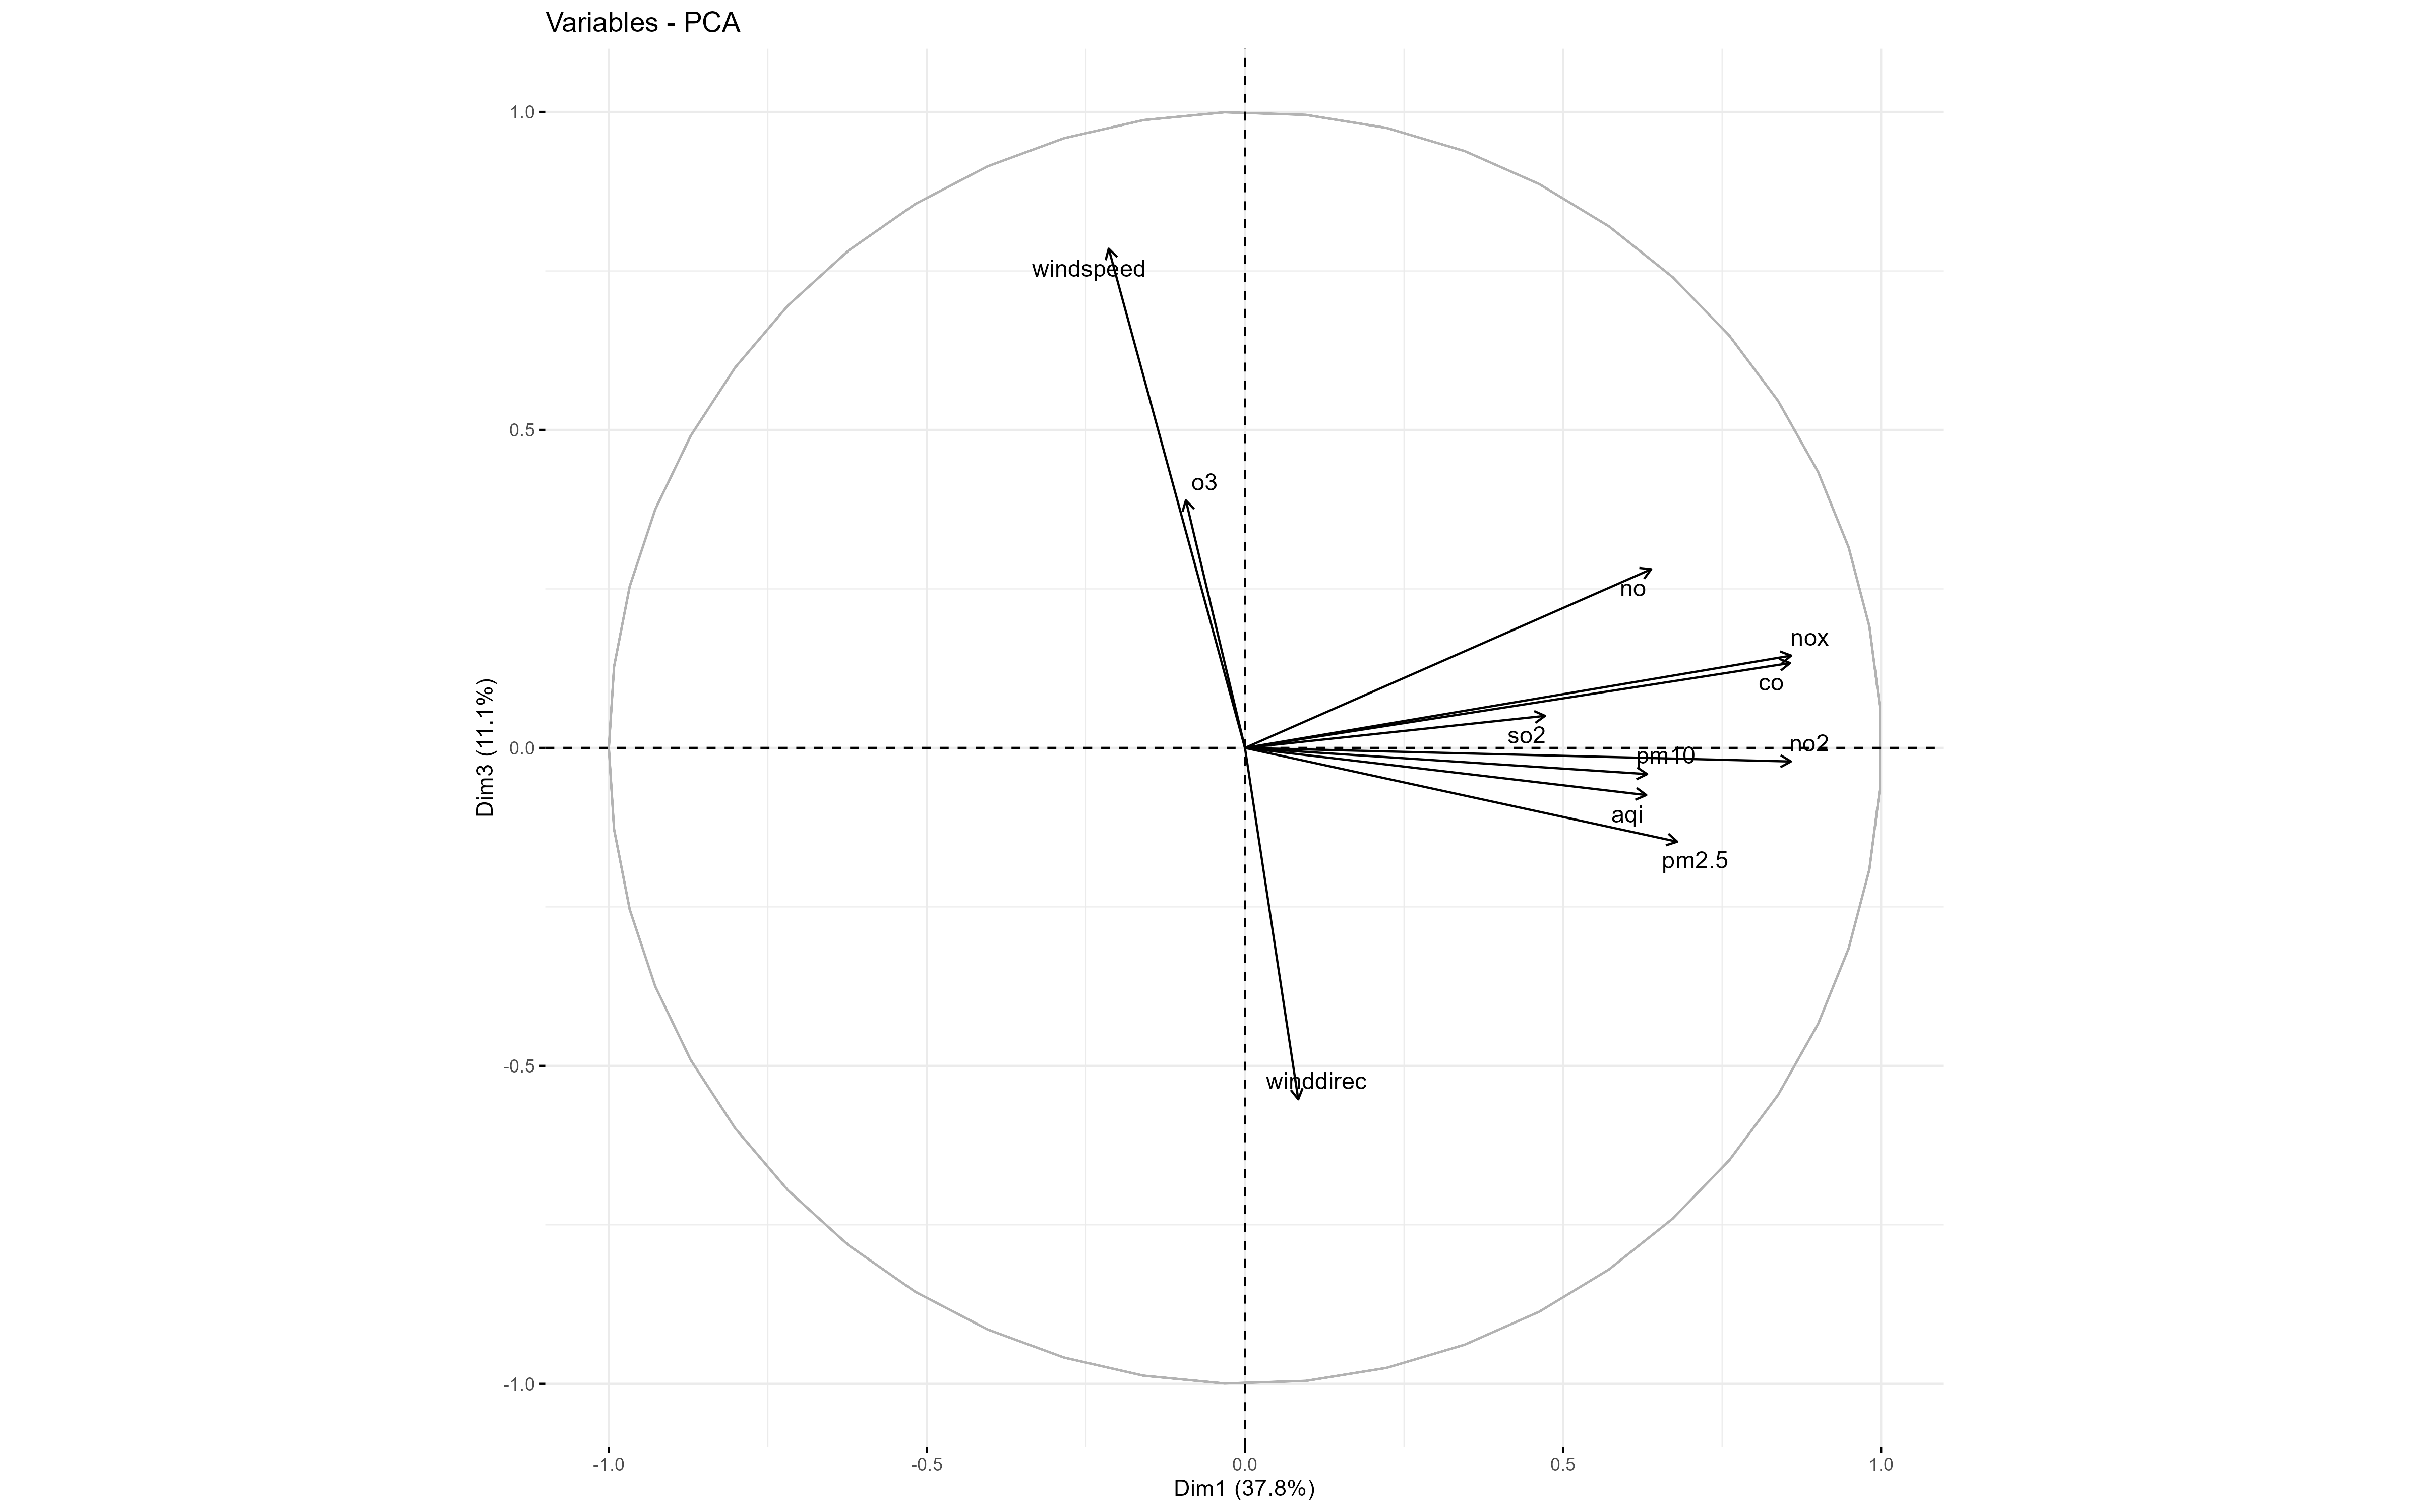
\includegraphics[height=2.8in]{plots/lab4/pca/projection-1-3.png}
\end{frame}

\begin{frame}
\frametitle{Аналіз головних компонент(Biplot)}
  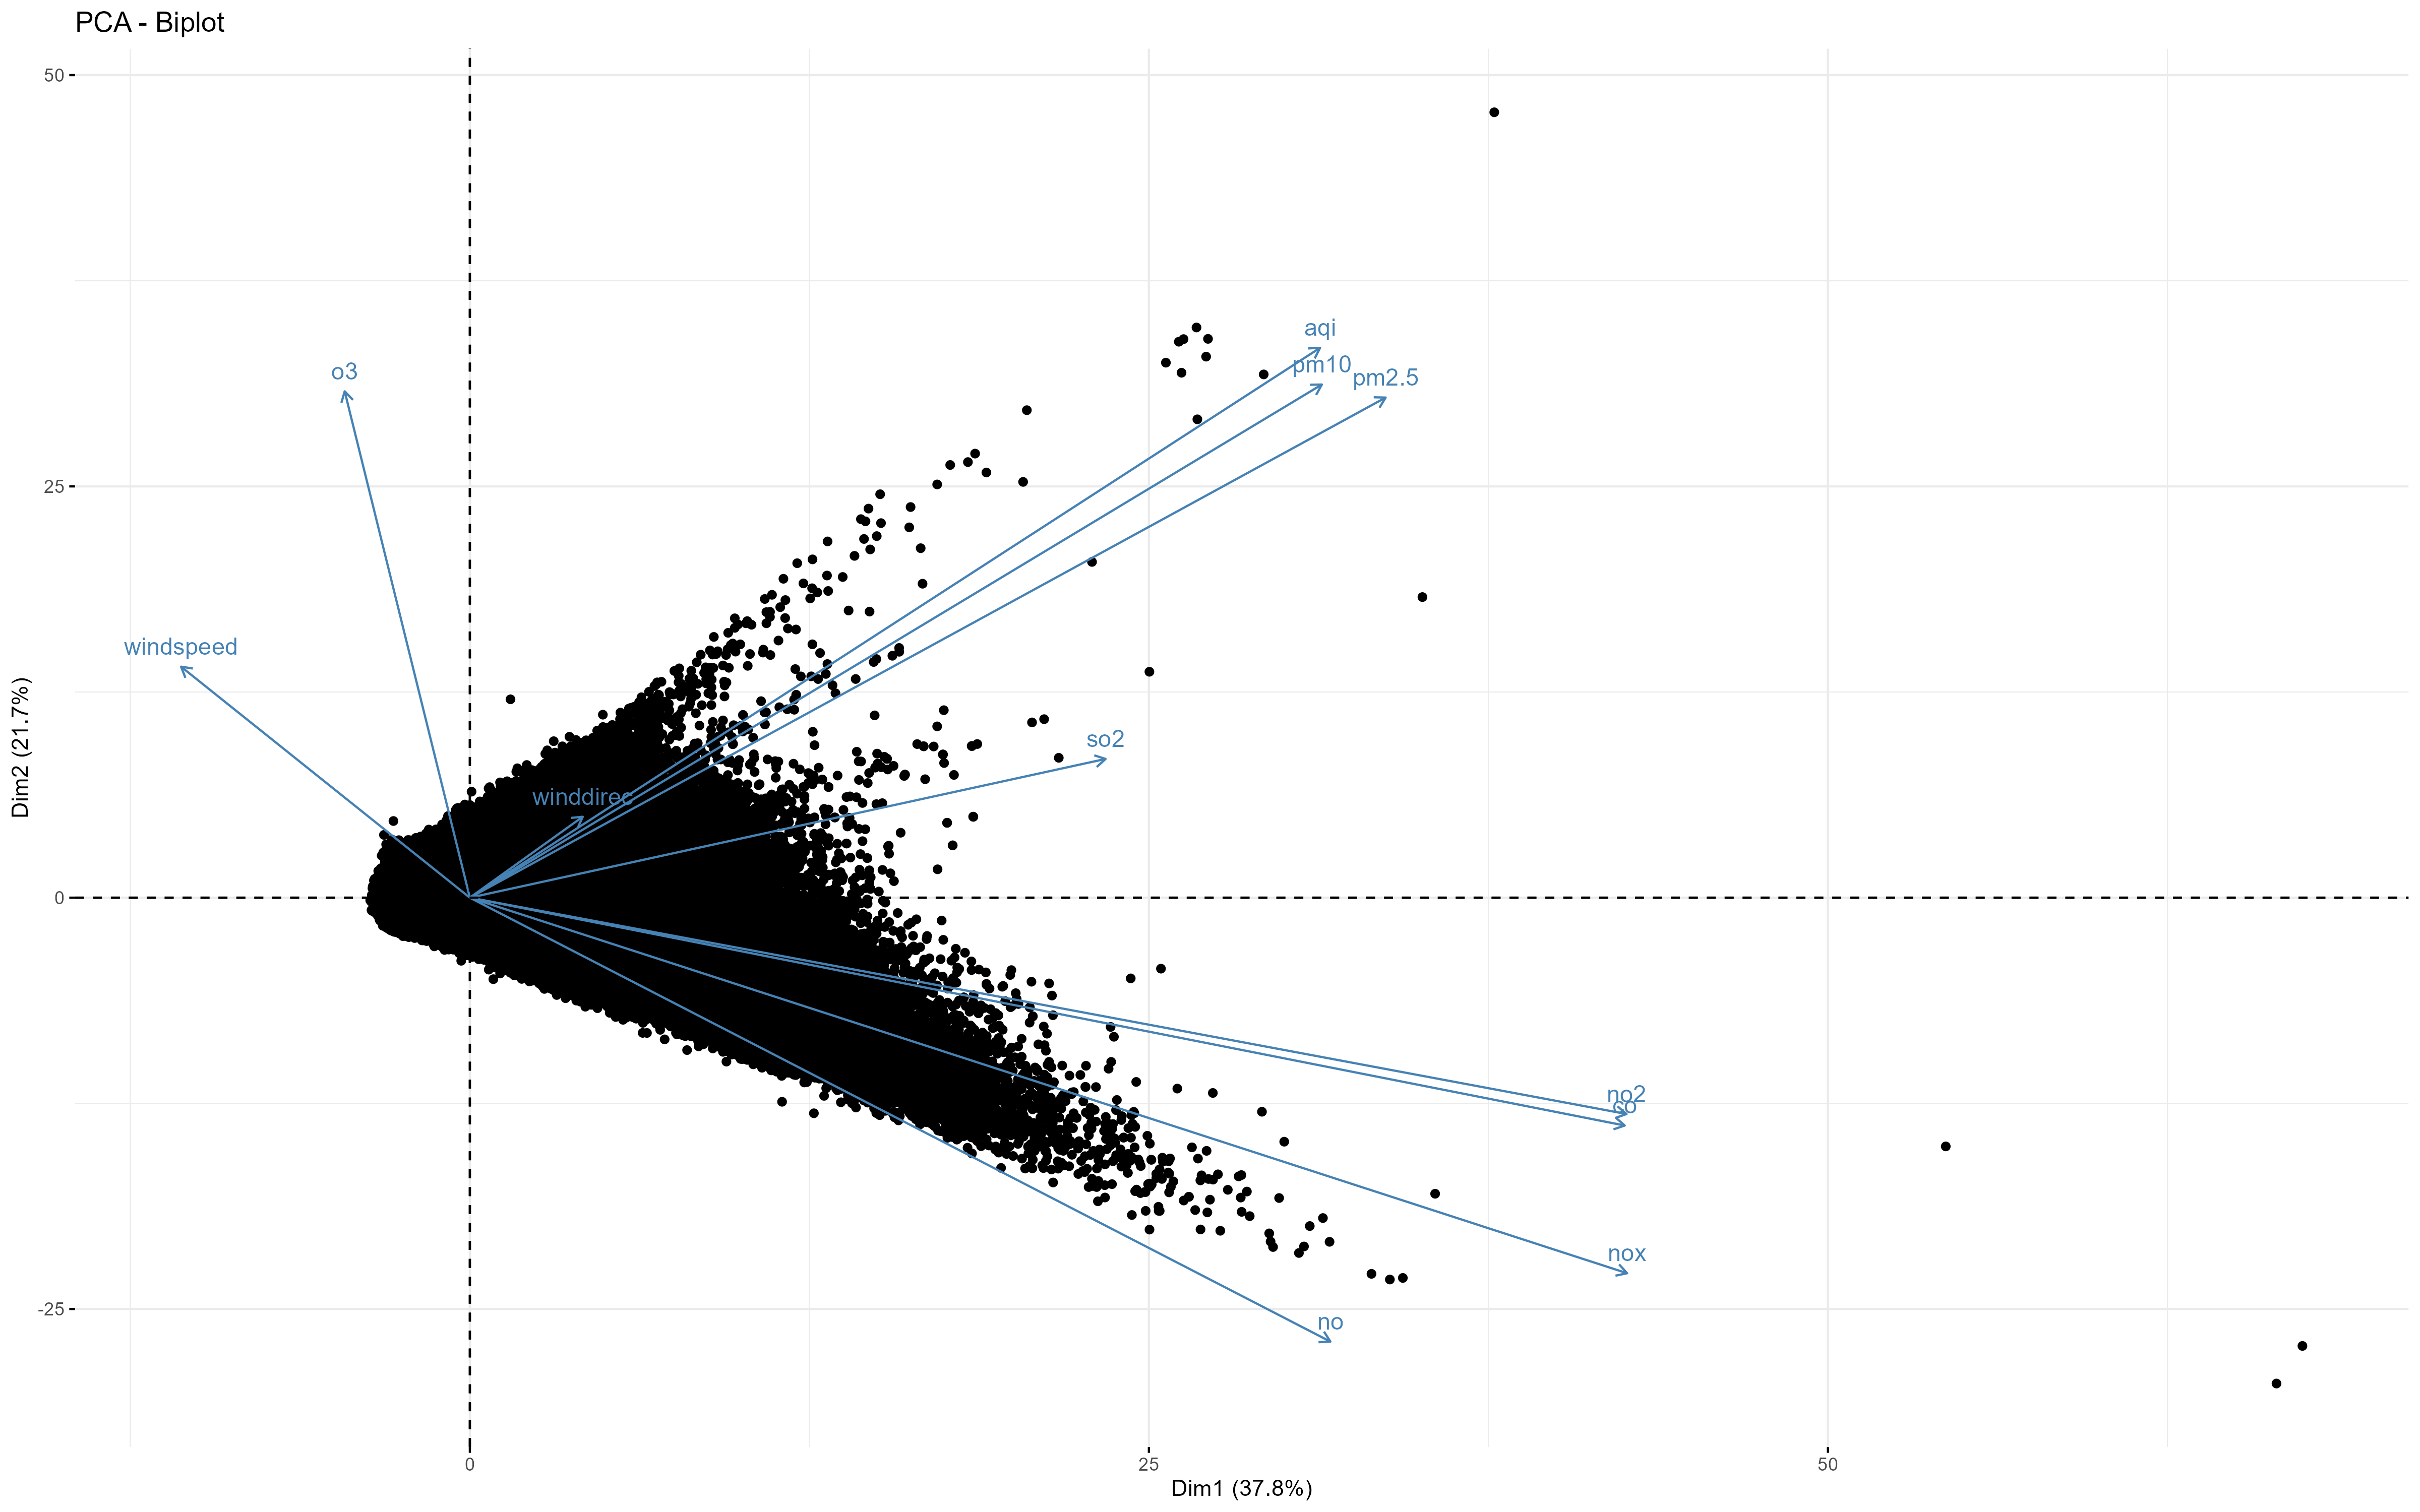
\includegraphics[height=2.8in]{plots/lab4/pca/biplot.png}
\end{frame}

\begin{frame}
  \frametitle{Висновок}
  \begin{itemize}
    \item Виявили ключові фактори, що визначають якість повітря,
     звівши складний набір даних до двох основних вимірів.
    \item Результати показують, що забруднювачі від транспорту/промисловості(домішки) діють спільно,
     а швидкість вітру є вирішальним фактором їх розсіювання.
  \end{itemize}
\end{frame}

\begin{frame}
  \section{Порівняня результатів}

  \frametitle{Зміст}
  \tableofcontents[currentsection]
\end{frame}

\begin{frame}
  \frametitle{Порівняння ЛР3 (параметрична) та ЛР4 (непараметрична)}
  
  \begin{ssmall}
  
  \begin{table}
  \centering
  \begin{talltblr}[         %% tabularray outer open
  entry=none,label=none,
  note{}={+ p \num{< 0.1}, * p \num{< 0.05}, ** p \num{< 0.01}, *** p \num{< 0.001}},
  ]                     %% tabularray outer close
  {                     %% tabularray inner open
  colspec={Q[]Q[]Q[]Q[]Q[]Q[]},
  column{2,3,4,5,6}={}{halign=c,},
  column{1}={}{halign=l,},
  hline{28}={1,2,3,4,5,6}{solid, black, 0.05em},
  }                     %% tabularray inner close
  \toprule
  & lin & np (1) & nppl (2.1) & nppl (2.2) & nppl (3) \\ \midrule %% TinyTableHeader
  reform\_days & \num{-0.010081}*** &  & \num{-0.009989}*** & \num{-0.010092}*** &  \\
  & (\num{0.000770}) &  & (\num{0.000342}) & (\num{0.000342}) &  \\
  jul\_days & \num{0.755704}*** &  &  &  &  \\
  & (\num{0.022698}) &  &  &  &  \\
  I(jul\_days\textasciicircum{}2) & \num{-0.002156}*** &  &  &  &  \\
  & (\num{0.000249}) &  &  &  &  \\
  windspeed & \num{-3.155031}*** &  & \num{-2.758367}*** & \num{-3.229516}*** & \num{-3.195055}*** \\
  & (\num{0.431494}) &  & (\num{0.255418}) & (\num{0.281014}) & (\num{0.254649}) \\
  after\_reform &  &  &  &  & \num{-17.638269}*** \\
  &  &  &  &  & (\num{0.631408}) \\ \midrule
  Num.Obs. & \num{7000} & 7000 & 7000 & 7000 & 7000 \\
  R2 & \num{0.469} & 0.40937 & 0.479709 & 0.485264 & 0.5449 \\
  RMSE & \num{23.22} & 24.696529 & 23.287205 & 23.110408 & 25.503944 \\
  \bottomrule
  \end{talltblr}
  \end{table} 
  
  \end{ssmall}
\end{frame}

\begin{frame}
  \section{Висновок}

  \frametitle{Зміст}
  \tableofcontents[currentsection]
\end{frame}

% Підсумувати основні результати непараметричного аналізу.
% - Які нелінійні залежності були виявлені та для яких змінних?
% - Як непараметричні моделі доповнили/змінили розуміння, отримане з параметричних моделей (ЛР3)?
% - Чи вдалося за допомогою PLM отримати збалансовану модель з інтерпретованими лінійними ефектами та гнучкою нелінійною компонентою?
% - Відповідь на головне питання дослідження: Як реформа покращення якості повітря вплинула на якість повітря, враховуючи нелінійності?
% - Обмеження дослідження та можливі напрямки для подальшої роботи.

\begin{frame}
  \frametitle{Висновок}
  
  В ході аналізу ми визначили, що:
  
   \begin{itemize}
    \item Ці моделі підтвердили значущий лінійний вплив реформи та швидкості вітру, але водночас виявивши складнішу природу сезонних коливань. 
    \item Частково-лінійна модель успішно поєднала інтерпретовані лінійні ефекти з гнучкою нелінійною компонентою, покращивши якість моделювання. 
    \item Реформа мала статистично значущий позитивний вплив, який проявлявся у поступовому зниженні AQI, навіть з урахуванням нелінійностей.
    \item Основним обмеженням залишається помірна пояснювальна здатність моделей, що вказує на потребу включення додаткових змінних у майбутньому.
  \end{itemize}
\end{frame}

\end{document}